%%%%%%%%%%%%%%%%%%%%%%%%%%%%%%%%%%%%%%%%%%%%%%%%%%%%%%%%%%%%%%%%%%%%%%%%%%%%%%
%
% MASTER FILE START
%
%%%%%%%%%%%%%%%%%%%%%%%%%%%%%%%%%%%%%%%%%%%%%%%%%%%%%%%%%%%%%%%%%%%%%%%%%%%%%%

\documentclass{beamer}
\usepackage{etex}
\mode<presentation> {
\usetheme{Singapore} 
\setbeamercovered{invisible}
\setbeamertemplate{navigation symbols}{} 
}
%%%%%%%%%%%%%%%%%%%%%%%%%%%%%%%%%%%%%%%%%%%%%%%%%%%%%%%%%%%%%%%%%%%%%%%%%%%%%%
%
% PACKAGES
%
%%%%%%%%%%%%%%%%%%%%%%%%%%%%%%%%%%%%%%%%%%%%%%%%%%%%%%%%%%%%%%%%%%%%%%%%%%%%%%
\newcommand\FrameText[1]{%
  \begin{textblock*}{\paperwidth}(261pt,239pt)
    \raggedright #1\hspace{.5em}
  \end{textblock*}}
\newcommand{\tikzmark}[1]{\tikz[overlay,remember picture] \node (#1) {};}
\graphicspath{{./figures/}}
\usepackage{cancel}
\usepackage{url}               % url typeset correctly
\usepackage{transparent}
\usepackage{named}
\usepackage{tikz}
\usepackage{picture}
\usepackage{algorithm,algorithmic}
\usepackage{multirow}
\usepackage{proof}
\usepackage{transparent}
\usepackage{url}
\usepackage{hyperref}	
\setlength{\inferLineSkip}{4pt}
%\usepackage[inference]{semantic}
\usetikzlibrary{shapes,arrows,snakes,backgrounds,%
matrix,patterns,arrows,decorations.pathmorphing,decorations.pathreplacing,%
positioning,fit,calc,decorations.text, automata%
}
\tikzset{%
  dots/.style args={#1per #2}{%
    line cap=round,
    dash pattern=on 0 off #2/#1
  }
}

\usepackage{color}
\newcommand{\hilightbl}[1]{\colorbox{darkblue!18}{#1}}
\newcommand{\hilightred}[1]{\colorbox{red!18}{#1}}
\usepackage{etoolbox}
\usepackage{tikz}
\newrobustcmd*{\myfilledtriangle}[1]{\tikz{\filldraw[draw=#1,fill=#1] (0,0) --
(0.2cm,0) -- (0.1cm,0.2cm);}}

\newrobustcmd*{\mytriangle}[2]{\tikz{\filldraw[very thick, dots=6 per 1cm, style=dotted,draw=#1,fill=#2] (0,0) --
(0.2cm,0) -- (0.1cm,0.2cm) -- (0,0);}}
\definecolor{lightblue}{HTML}{D4E1F5}
\definecolor{darkred}{HTML}{632E2E}


\newcommand{\call}{\ensuremath{%
  \mathchoice{\includegraphics[height=5ex]{call3}}
    {\includegraphics[height=4ex]{call3}}
    {\includegraphics[height=3ex]{call3}}
    {\includegraphics[height=2.5ex]{call3}}
}}

\newcommand{\sups}{\ensuremath{%
  \mathchoice{
\includegraphics[height=1.1ex]{supset}}
    {
\includegraphics[height=1.1ex]{supset}}
    {
\includegraphics[height=0.6ex]{supset}}
    {
\includegraphics[height=0.6ex]{supset}}
}}



\newcommand{\rf}{\ensuremath{%
  \mathchoice{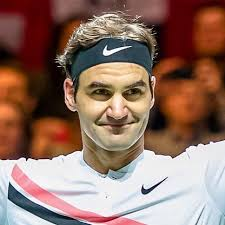
\includegraphics[height=14ex]{rf}}
    {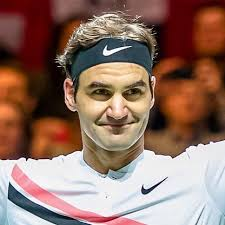
\includegraphics[height=13ex]{rf}}
    {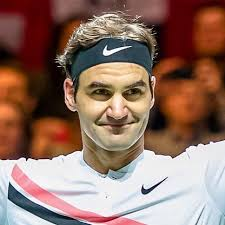
\includegraphics[height=12ex]{rf}}
    {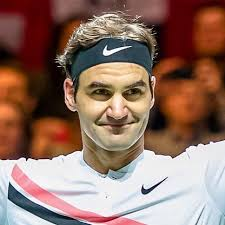
\includegraphics[height=11.5ex]{rf}}
}}


\newcommand{\rfo}{\ensuremath{%
  \mathchoice{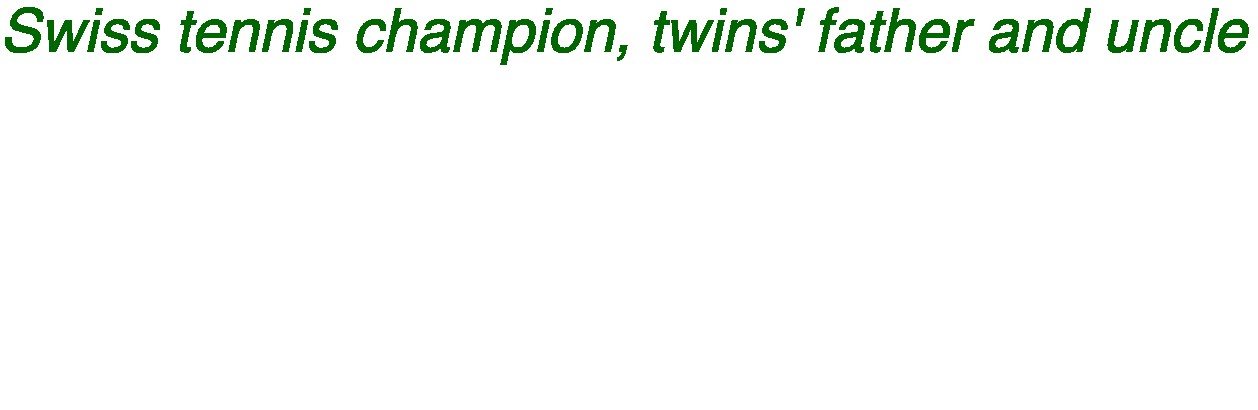
\includegraphics[height=14ex]{rf2}}
    {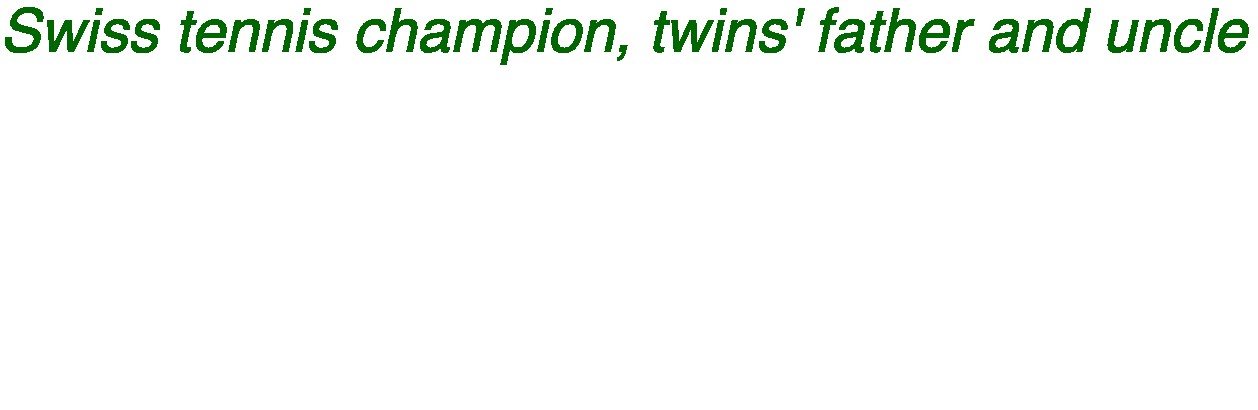
\includegraphics[height=13ex]{rf2}}
    {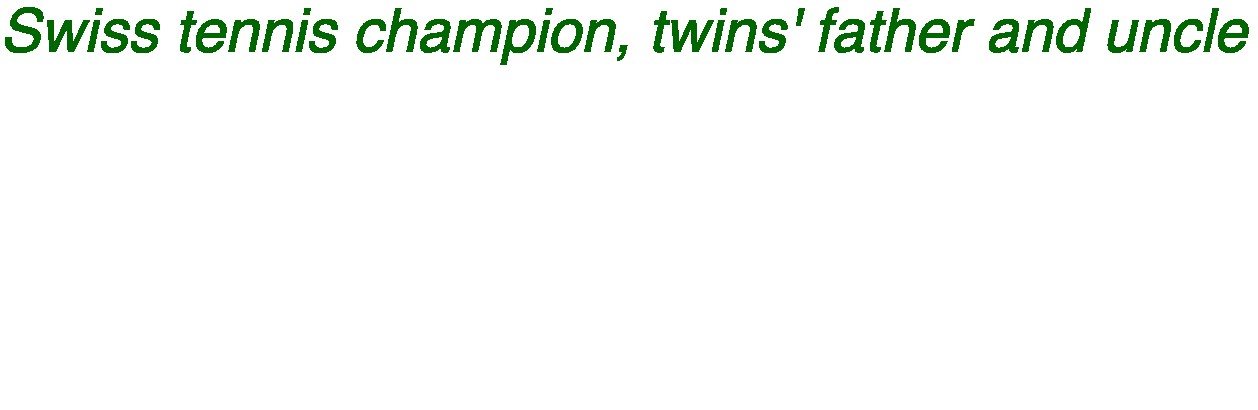
\includegraphics[height=12ex]{rf2}}
    {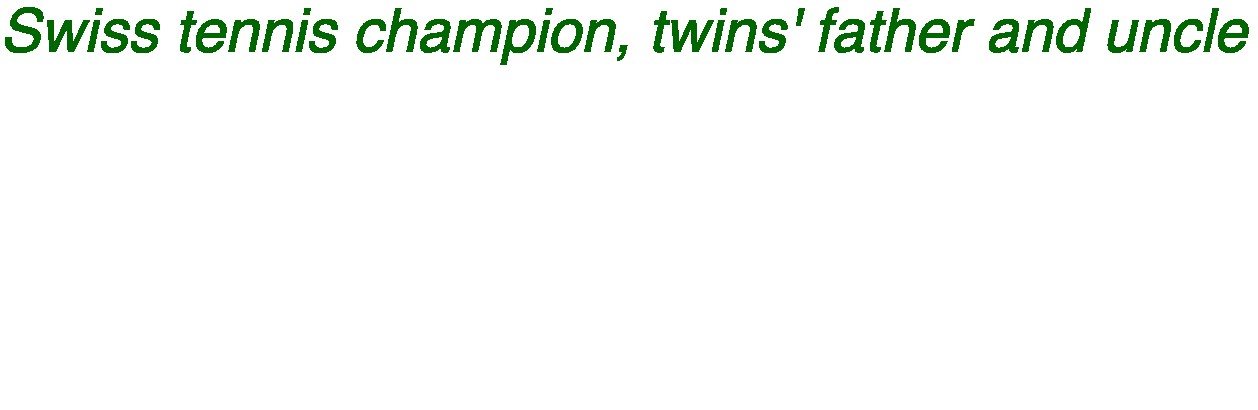
\includegraphics[height=11.5ex]{rf2}}
}}



\definecolor{gray}{rgb}{0.4,0.4,0.4}
\definecolor{darkblue}{rgb}{0.0,0.0,0.6}
\definecolor{cyan}{rgb}{0.0,0.6,0.6}
\definecolor{darkgreen}{rgb}{0,0.4,0}
\def\checkmark{\tikz\fill[scale=0.4](0,.35) -- (.25,0) -- (1,.7) -- (.25,.15) -- cycle;} 
\setbeamertemplate{blocks}[rounded][shadow=false]

%%% Grid on the slides

% \usepackage[texcoord,grid,gridunit=mm,gridcolor=red!10,subgridcolor=green!10]
% {eso-pic}

\usepackage{enumerate}
\usepackage{amstext}
\usepackage{amssymb}
\usepackage{amsbsy}
\usepackage{amsmath}
\usepackage{color}
\usepackage[absolute,overlay]{textpos}
\usepackage{cancel}

\mode<article>
{
\usepackage{fullpage}
}

\def\uminus{\setbox0=\hbox{$\cup$}\rlap{\hbox
    to\wd0{\hss\raise0.3ex\hbox{$\scriptscriptstyle{-}$}\hss}}\box0}
\def\cminus{\setbox0=\hbox{$\cap$}\rlap{\hbox
    to\wd0{\hss\raise0.3ex\hbox{$\scriptscriptstyle{-}$}\hss}}\box0}
\definecolor{light-gray}{gray}{0.45}

\usepackage{soul}




%%%%%%%%%%%%%%%%%%%%%%%%%%%%%%%%%%%%%%%%%%%%%%%%%%%%%%%%%%%%%%%%%%%%%%%%%%%%%%
%
% CUSTOM BEAMER STYLE
%
%%%%%%%%%%%%%%%%%%%%%%%%%%%%%%%%%%%%%%%%%%%%%%%%%%%%%%%%%%%%%%%%%%%%%%%%%%%%%
\setbeamertemplate{blocks}[rounded][shadow=false]
% setup margin
\beamersetleftmargin{0.5cm}
\beamersetrightmargin{0.5cm}

% setup symbols
\setbeamertemplate{bibliography item}[book]
\setbeamertemplate{navigation symbols}{} % turn off navigation symbols

% setup font shapes of various elements
\setbeamerfont{frametitle}{series=\bfseries}
%\setbeamercolor{alerted text}{series=\bfseries}

% put number of frames at the bottom
\setbeamertemplate{footline}[frame number]


\usepackage[scaled]{helvet}

\newtheorem{proposition}[theorem]{Proposition}


\setbeamercolor{alerted text}{fg=purple}

\newcommand{\makeoverview}{%
  \begin{frame}
    \frametitle{Overview}
    \tableofcontents
  \end{frame}
}

\newcommand{\makereferences}[1]{%
  \begin{frame}[allowframebreaks,allowdisplaybreaks]
    \frametitle{References}
    \bibliography{#1}
  \end{frame}
}



%%%%%%%%%%%%%% SPACING COMMANDS 

\newcommand{\bs}{\bigskip}
\newcommand{\m}{\medskip}
\newcommand{\s}{\smallskip}
\newcommand{\cG}{\ensuremath{\mathcal{G}}}

%%%%%%%%%%%%%% SPECIFIC MACROS
\newcommand{\weak}{\ensuremath{\mathit{weak}}}
\newcommand{\FLP}{\ensuremath{\mathit{flp}}}
\newcommand{\wred}[3]{\ensuremath{{#1^{#2,#3}_{\mi{weak}}}}}
\newcommand{\flpred}[3]{\ensuremath{{#1^{#2,#3}_{\mi{flp}}}}}
\newcommand{\citeY}[1]{\citeyear{#1}}
\newcommand{\naf}{{\it not}\,}
\newcommand{\NP}{\ensuremath{\mathrm{NP}}}
\newcommand{\SigmaP}[1]{{\Sigma}_{#1}^{P}}
\newcommand{\wrt}[0]{w.r.t.\ }
\newcommand{\tuple}[1]{\ensuremath{\langle#1\rangle}}
\renewcommand{\vec}[1]{\ensuremath{\mathbf{#1}}}
\newcommand{\dlliteplugin}{{\fontencoding{OT1}\fontfamily{cmss}\selectfont{dlliteplugin}}}
\newcommand{\hnbls}{\vspace*{-.5\baselineskip}}
\newcommand{\bl}[1]{\textcolor{blue}{#1}}
\newcommand{\prg}{\mathcal{P}}
\newcommand{\gr}[1]{\textcolor{darkgreen}{#1}}
\newcommand{\dllite}{\ensuremath{DL}\text{-}\ensuremath{Lite}}
\newcommand{\el}{\ensuremath{\mathcal{EL}}}
\newcommand{\specialcell}[2][l]{\begin{tabular}[#1]{@{}c@{}}#2\end{tabular}}
   \newcommand*\circled[1]{%
      \tikz[baseline=(C.base)]\node[draw,circle,fill=red!10,inner sep=1.7pt](C) {#1};\!
    }
   \newcommand*\circledbl[1]{%
      \tikz[baseline=(C.base)]\node[draw,circle,fill=blue!10,inner sep=1.7pt](C) {#1};\!
    }

\usepackage{color}
\newcommand{\hilight}[1]{\colorbox{blue!18}{#1}}

\setbeamercolor{uppercolblue}{fg=black,bg=darkblue!15}
\setbeamercolor{lowercolblue}{fg=black,bg=darkblue!0}

\setbeamercolor{uppercolgreen}{fg=black,bg=darkgreen!15}
\setbeamercolor{lowercolgreen}{fg=black,bg=darkgreen!7}

\setbeamercolor{uppercolred}{fg=black,bg=red!15}
\setbeamercolor{lowercolred}{fg=black,bg=red!7}

\def\cA{\ensuremath{\mathcal{A}}}
\def\cT{\ensuremath{\mathcal{T}}}
\def\cI{\ensuremath{\mathcal{I}}}
\def\cC{\ensuremath{\mathcal{C}}}
\def\cO{\ensuremath{\mathcal{O}}}
\def\cR{\ensuremath{\mathcal{R}}}
\def\cP{\ensuremath{\mathcal{P}}}
\newcommand{\dlvhex}{\textsf{dlvhex}}
\usepackage{appendixnumberbeamer}


\newcommand\hex{{\sc hex}}

\catcode`\@=11 % as in plain.tex
\long\def\blank#1{\bl@nk#1@@..\bl@nk}%
\long\def\bl@nk#1#2@#3#4\bl@nk{#3#4}
\catcode`\@=12

\long\def\test#1{\begingroup \toks0{[#1]}%
  \newlinechar`\/\message{/\the\toks0:
  \if\blank{#1}EMPTY\else NOT empty\fi%
}\endgroup}



\newcommand{\mi}[1]{\ensuremath{\mathit{#1}}}
\newcommand{\mb}[1]{\ensuremath{\mathbf{#1}}}
\newcommand{\tbf}[1]{\textbf{#1}}
\newcommand{\dlatom}[3]{\ensuremath{{\operatorname{DL}}{[#1;#2]}{(#3)}}}


%%%%%%%%%%%%%%%%%%%%%%%%%%%%%%%%%%%%%%%%%%%%%%%%%%%%%%%%%%%%%%%%%%%%%%%%%%%%%%
%
% DOCUMENT PROPERTIES
%
%%%%%%%%%%%%%%%%%%%%%%%%%%%%%%%%%%%%%%%%%%%%%%%%%%%%%%%%%%%%%%%%%%%%%%%%%%%%%%



\title{Rule Induction and Reasoning over Knowledge Graphs}
 \author[Stepanova, Gad-Elrab, Vinh Ho]
 {
 }

 \titlegraphic{
  \centering

\includegraphics[height=1.3cm]{logo_mpi_430}

}

\date{26.09.2018}


%%%%%%%%%%%%%%%%%%%%%%%%%%%%%%%%%%%%%%%%%%%%%%%%%%%%%%%%%%%%%%%%%%%%%%%%%%%%%%
%
% DOCUMENT START
%
%%%%%%%%%%%%%%%%%%%%%%%%%%%%%%%%%%%%%%%%%%%%%%%%%%%%%%%%%%%%%%%%%%%%%%%%%%%%%%


\begin{document}

\frame{\titlepage}


\addtocounter{framenumber}{-1}

\makeoverview

%%%%%%%%%%%%%%%%%%%%%%%%%%%%%%%%%%%%%%%%%%%%%%%%%%%%%%%%%%%%%%%%%%%%%%%%%%%%%%


\section{Motivation}

\subsection{Knowledge Graphs}
\begin{frame}\frametitle{Knowledge Graphs}
\end{frame}
\begin{frame}\frametitle{Applications of KGs}
\end{frame}
\begin{frame}\frametitle{Issues}
\end{frame}
\subsection{Rules}
\begin{frame}\frametitle{Rules and Reasoning}
\end{frame}
\section{ILP}
\begin{frame}\frametitle{Main Motivation}
\end{frame}
\begin{frame}\frametitle{Foundation}
\end{frame}
\begin{frame}\frametitle{Technical Details}
\end{frame}

\section{Learning Rules from KGs}
\subsection{AMIE and other Systems}
\begin{frame}
\frametitle{Itemset Mining}
\end{frame}
\begin{frame}
\frametitle{Relational Pattern Mining}
\end{frame}
\section{Exception-awareness}
\begin{frame}
\frametitle{Shortcomings of Horn Rule Learning}
\end{frame}
\begin{frame}
\frametitle{Example}
\end{frame}
\begin{frame}
\frametitle{Approach Descriptions}
\end{frame}
\section{Completeness-awareness}
\begin{frame}
\frametitle{Approach Description}
\end{frame}
\section{Rules from Hybrid Sources}
\begin{frame}
\frametitle{Approach Description}
\end{frame}

% \section{Motivation}
% \begin{frame}\frametitle{\alt<3>{What is Digital Knowledge?}{What is Knowledge?}}
% \centerline{\alt<3>{\emph{``\bl{Digital knowledge} is semantically enriched machine processable data''}}{Plato: \emph{``\bl{Knowledge} is justified true belief''}}}
% \bigskip
% \bigskip
% \bigskip
% \bigskip
% \bigskip
% \bigskip
% \bigskip
% \bigskip
% \bigskip
% \bigskip
% \bigskip
% \bigskip
% \bigskip
% \bigskip
% \bigskip
% \bigskip

% \alt<3>{\begin{picture}(0.5,0.5)
% \put(45,-22){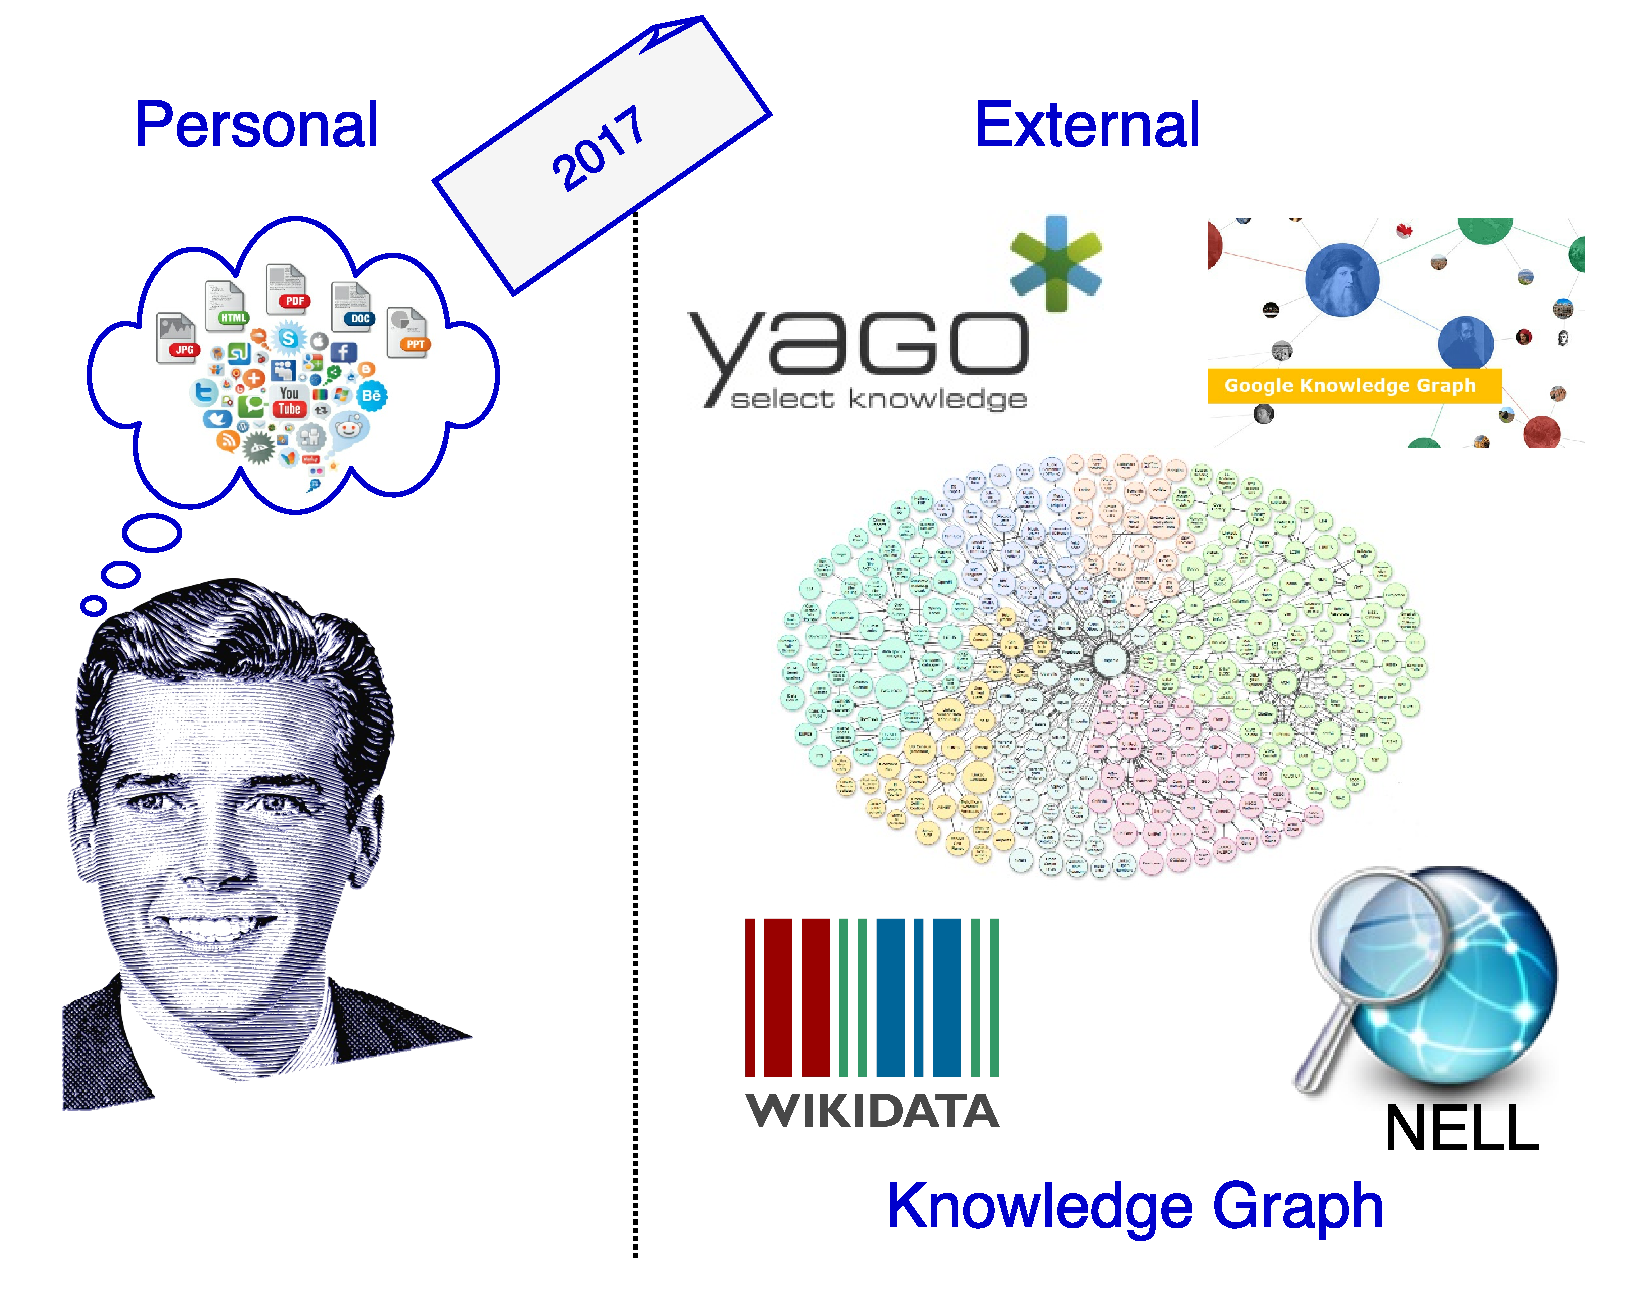
\includegraphics[width=.78\textwidth]{know3_}}
% \end{picture}}{\alt<2>{\begin{picture}(0.5,0.5)
% \put(45,-22){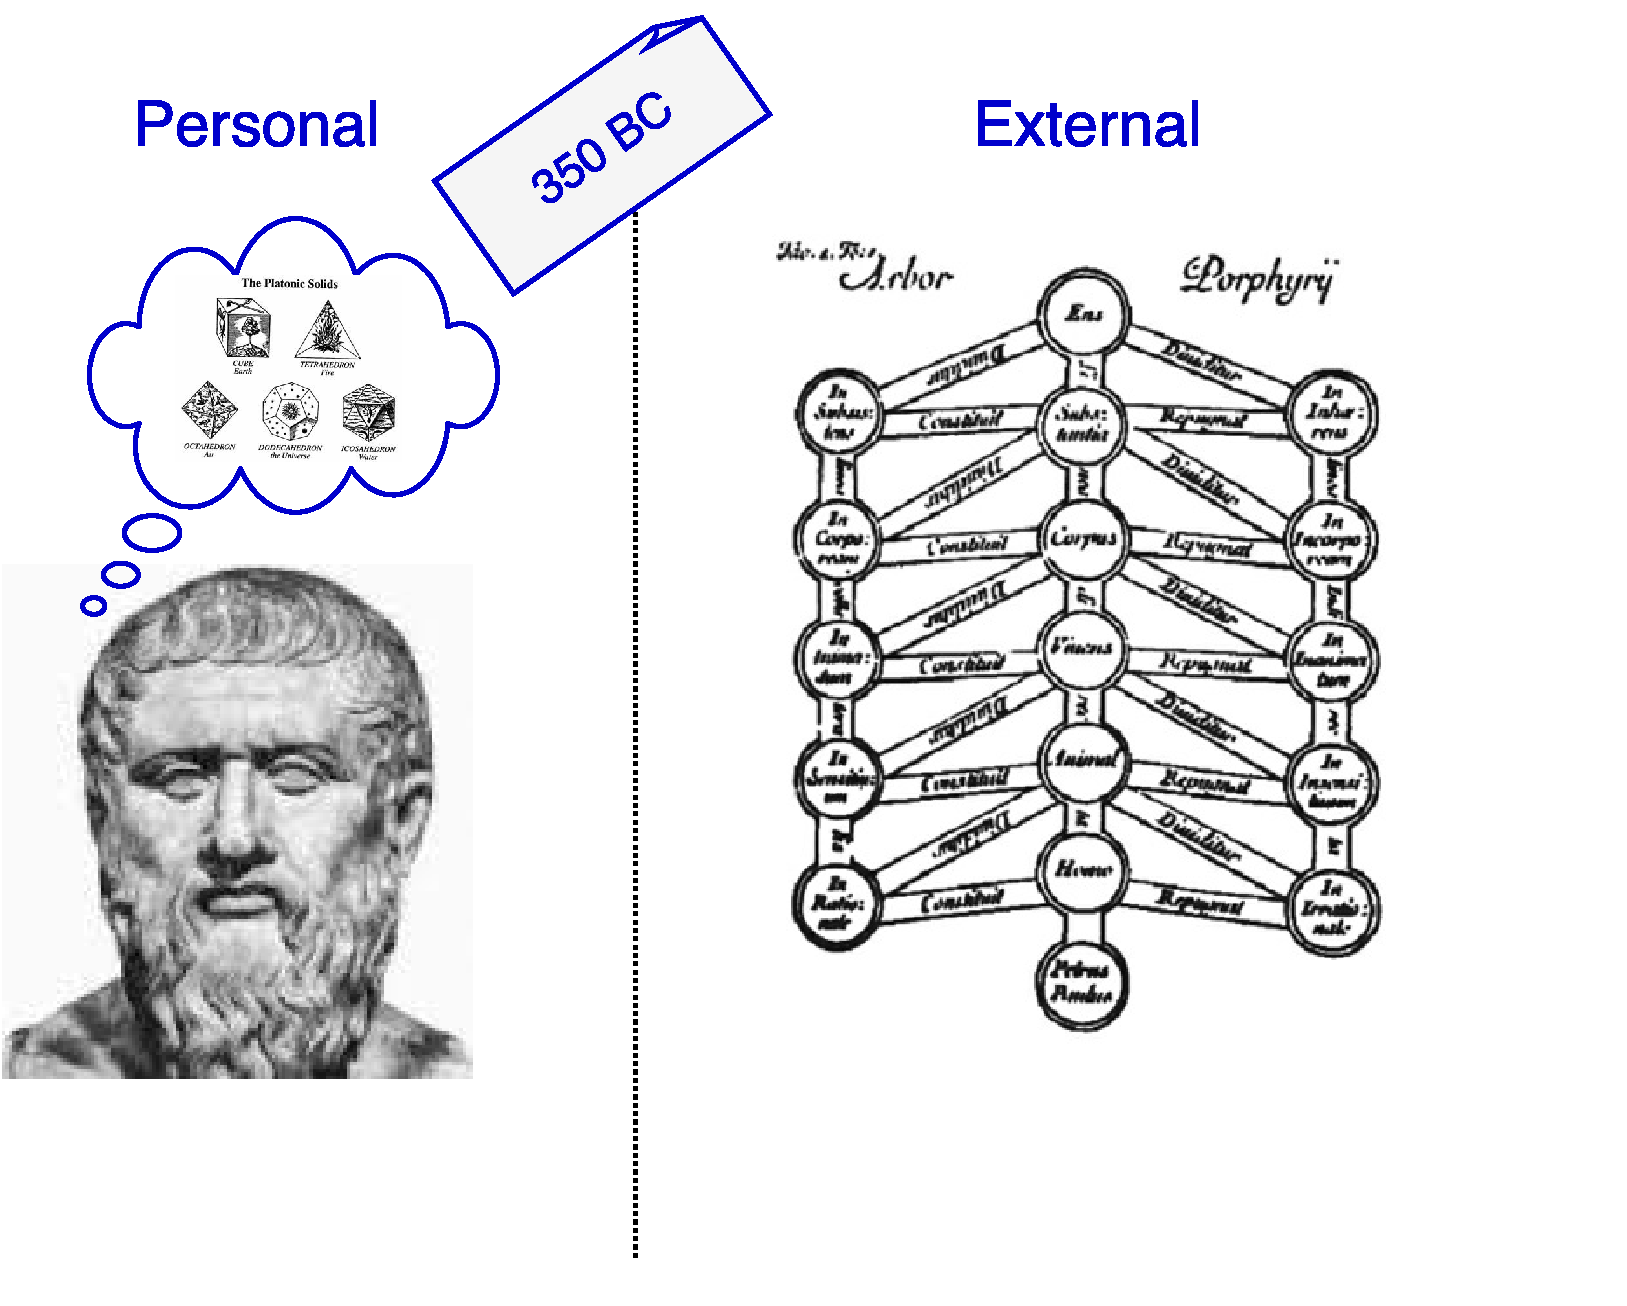
\includegraphics[width=.78\textwidth]{know1}}
% \end{picture}}{\begin{picture}(0.5,0.5)
% \put(45,-22){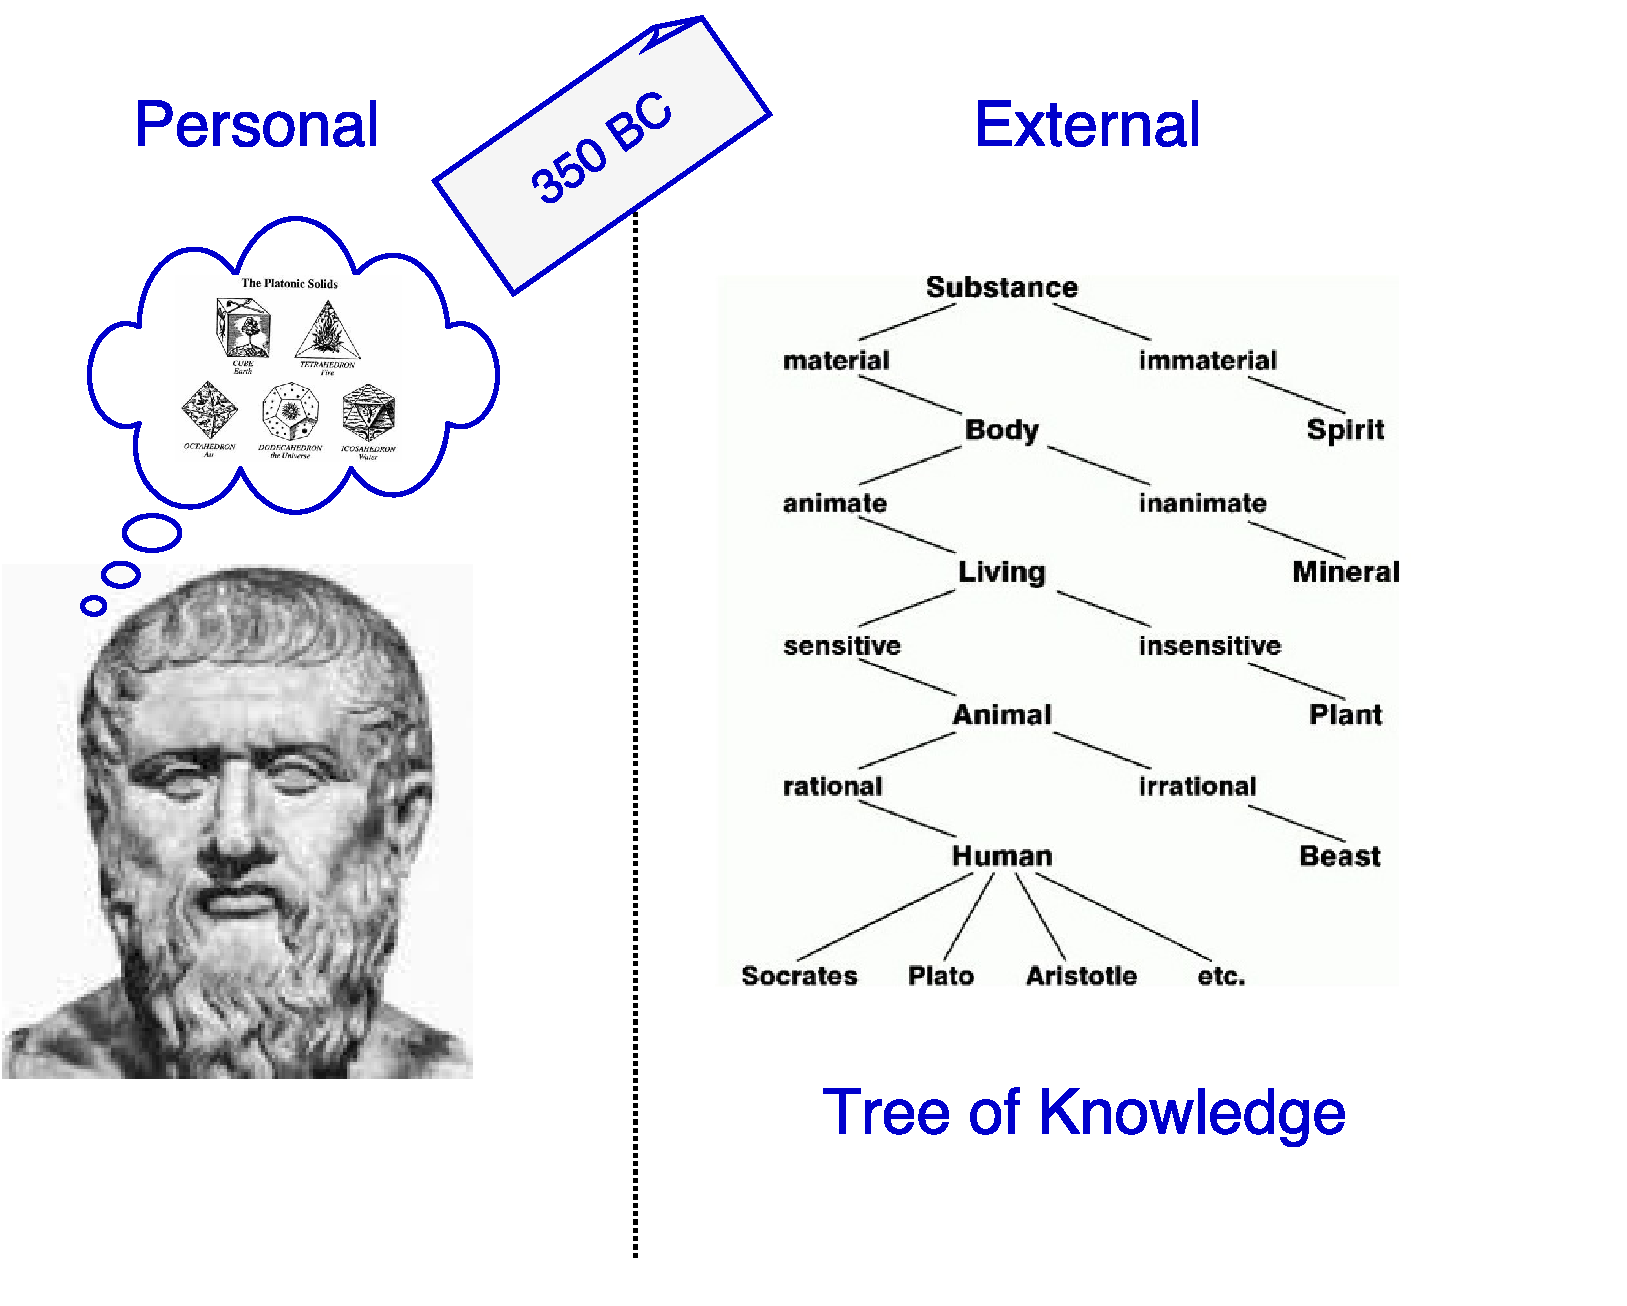
\includegraphics[width=.78\textwidth]{know2}}
% \end{picture}}
% }
% \end{frame}


% \begin{frame}\frametitle{Semantic Web Search}

% \alt<3>{\begin{picture}(0.5,0.5)
% \put(-13,-125){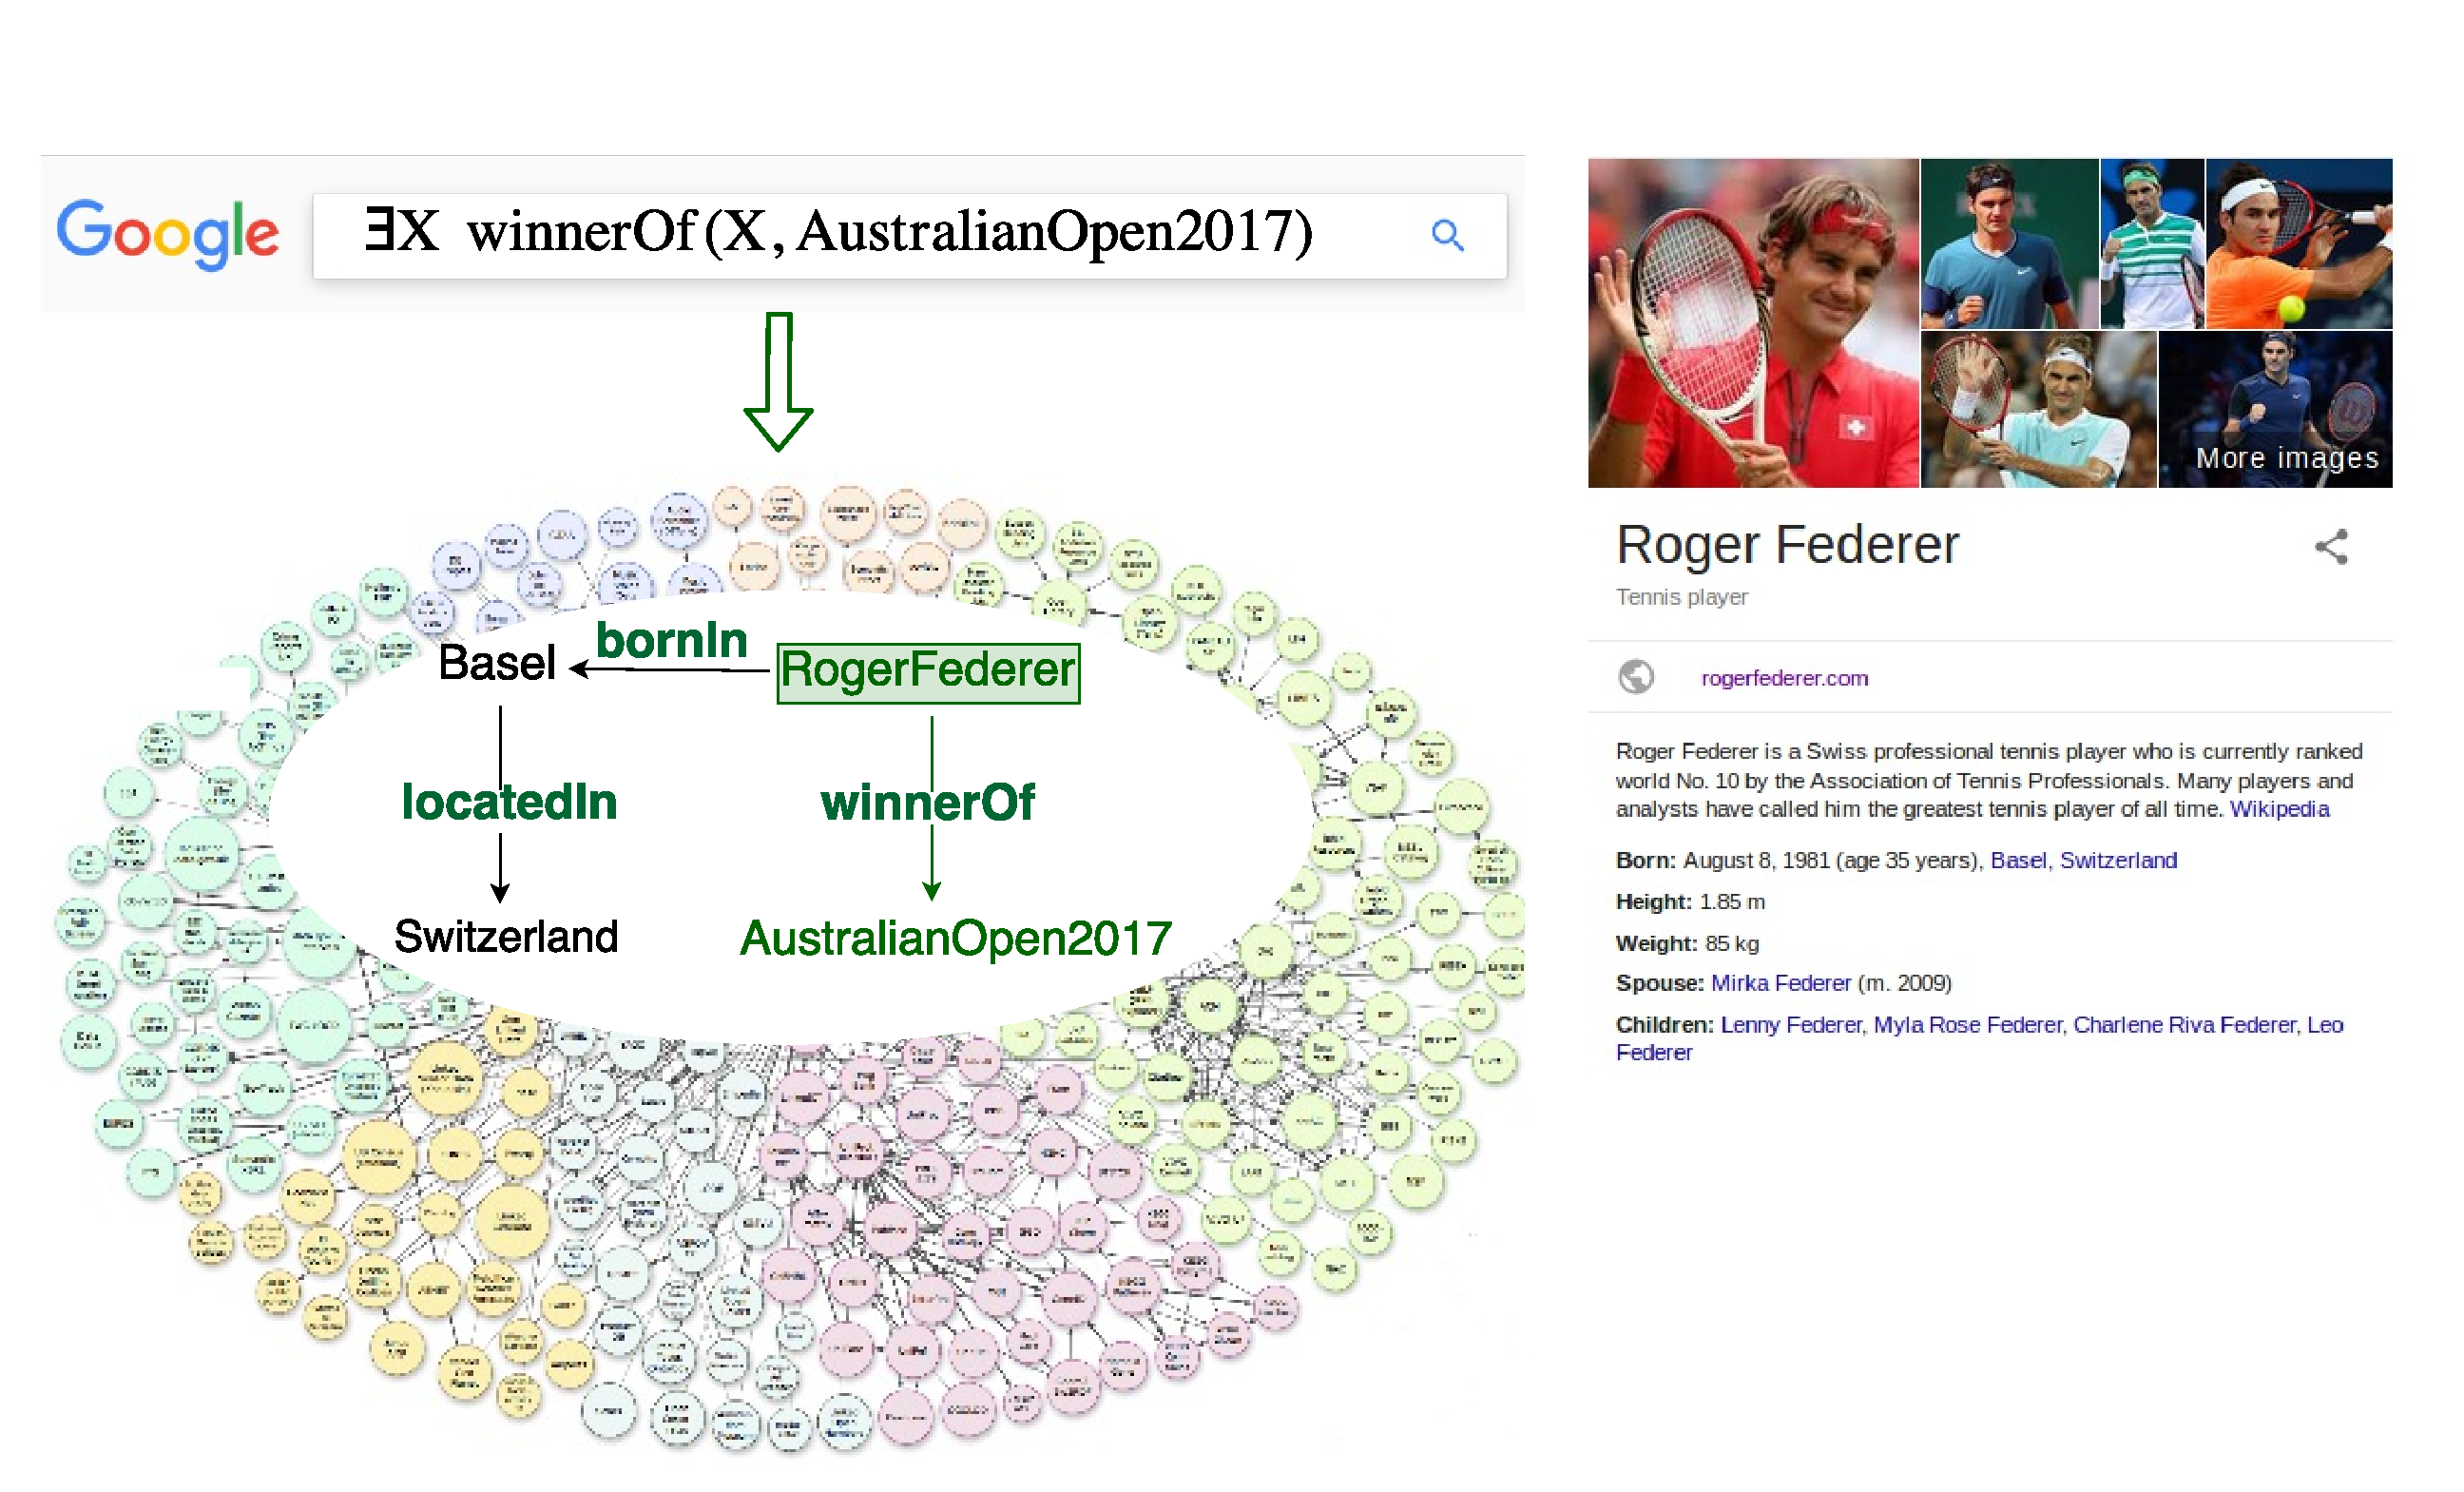
\includegraphics[width=1.1\textwidth]{semsearch3}}
% \end{picture}}{
% \alt<2>{\begin{picture}(0.5,0.5)
% \put(-13,-125){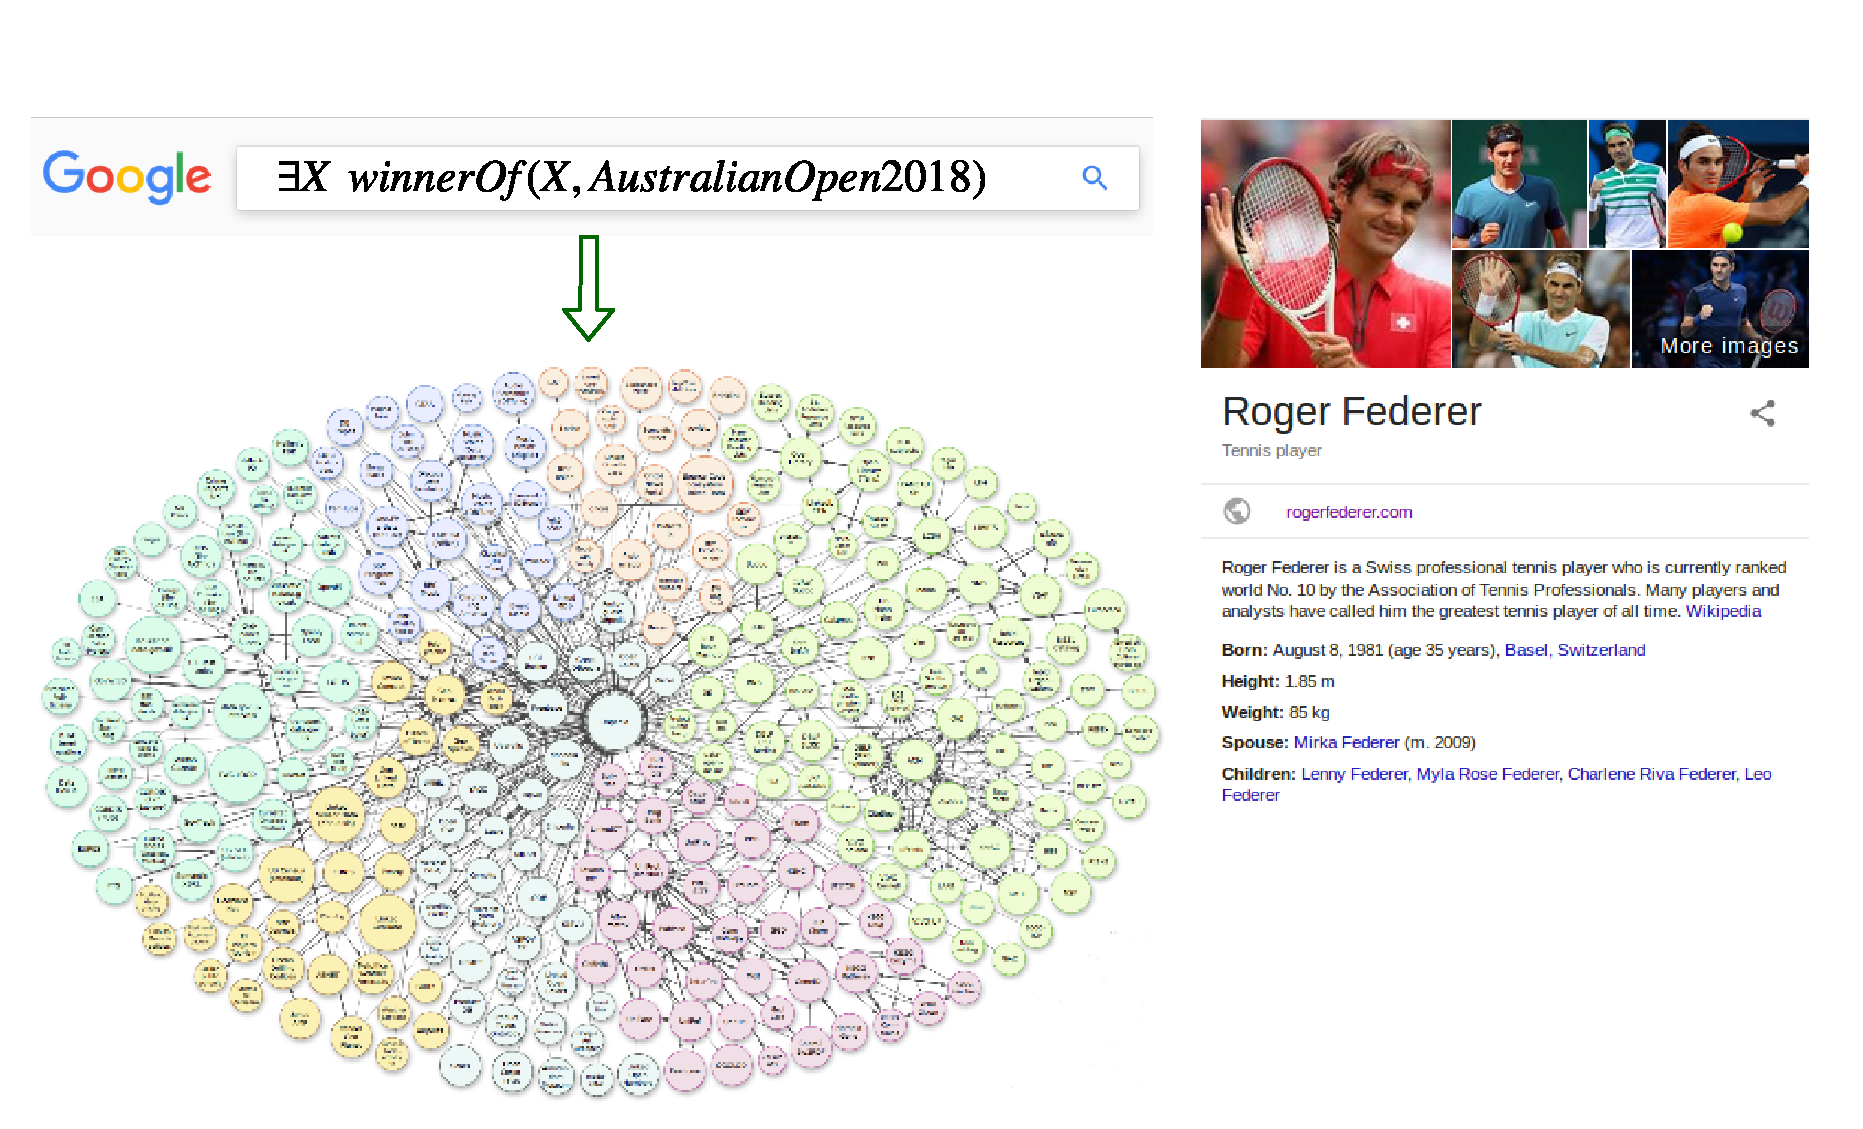
\includegraphics[width=1.1\textwidth]{semsearch2}}
% \end{picture}}{
% \begin{picture}(0.5,0.5)
% \put(-13,-125){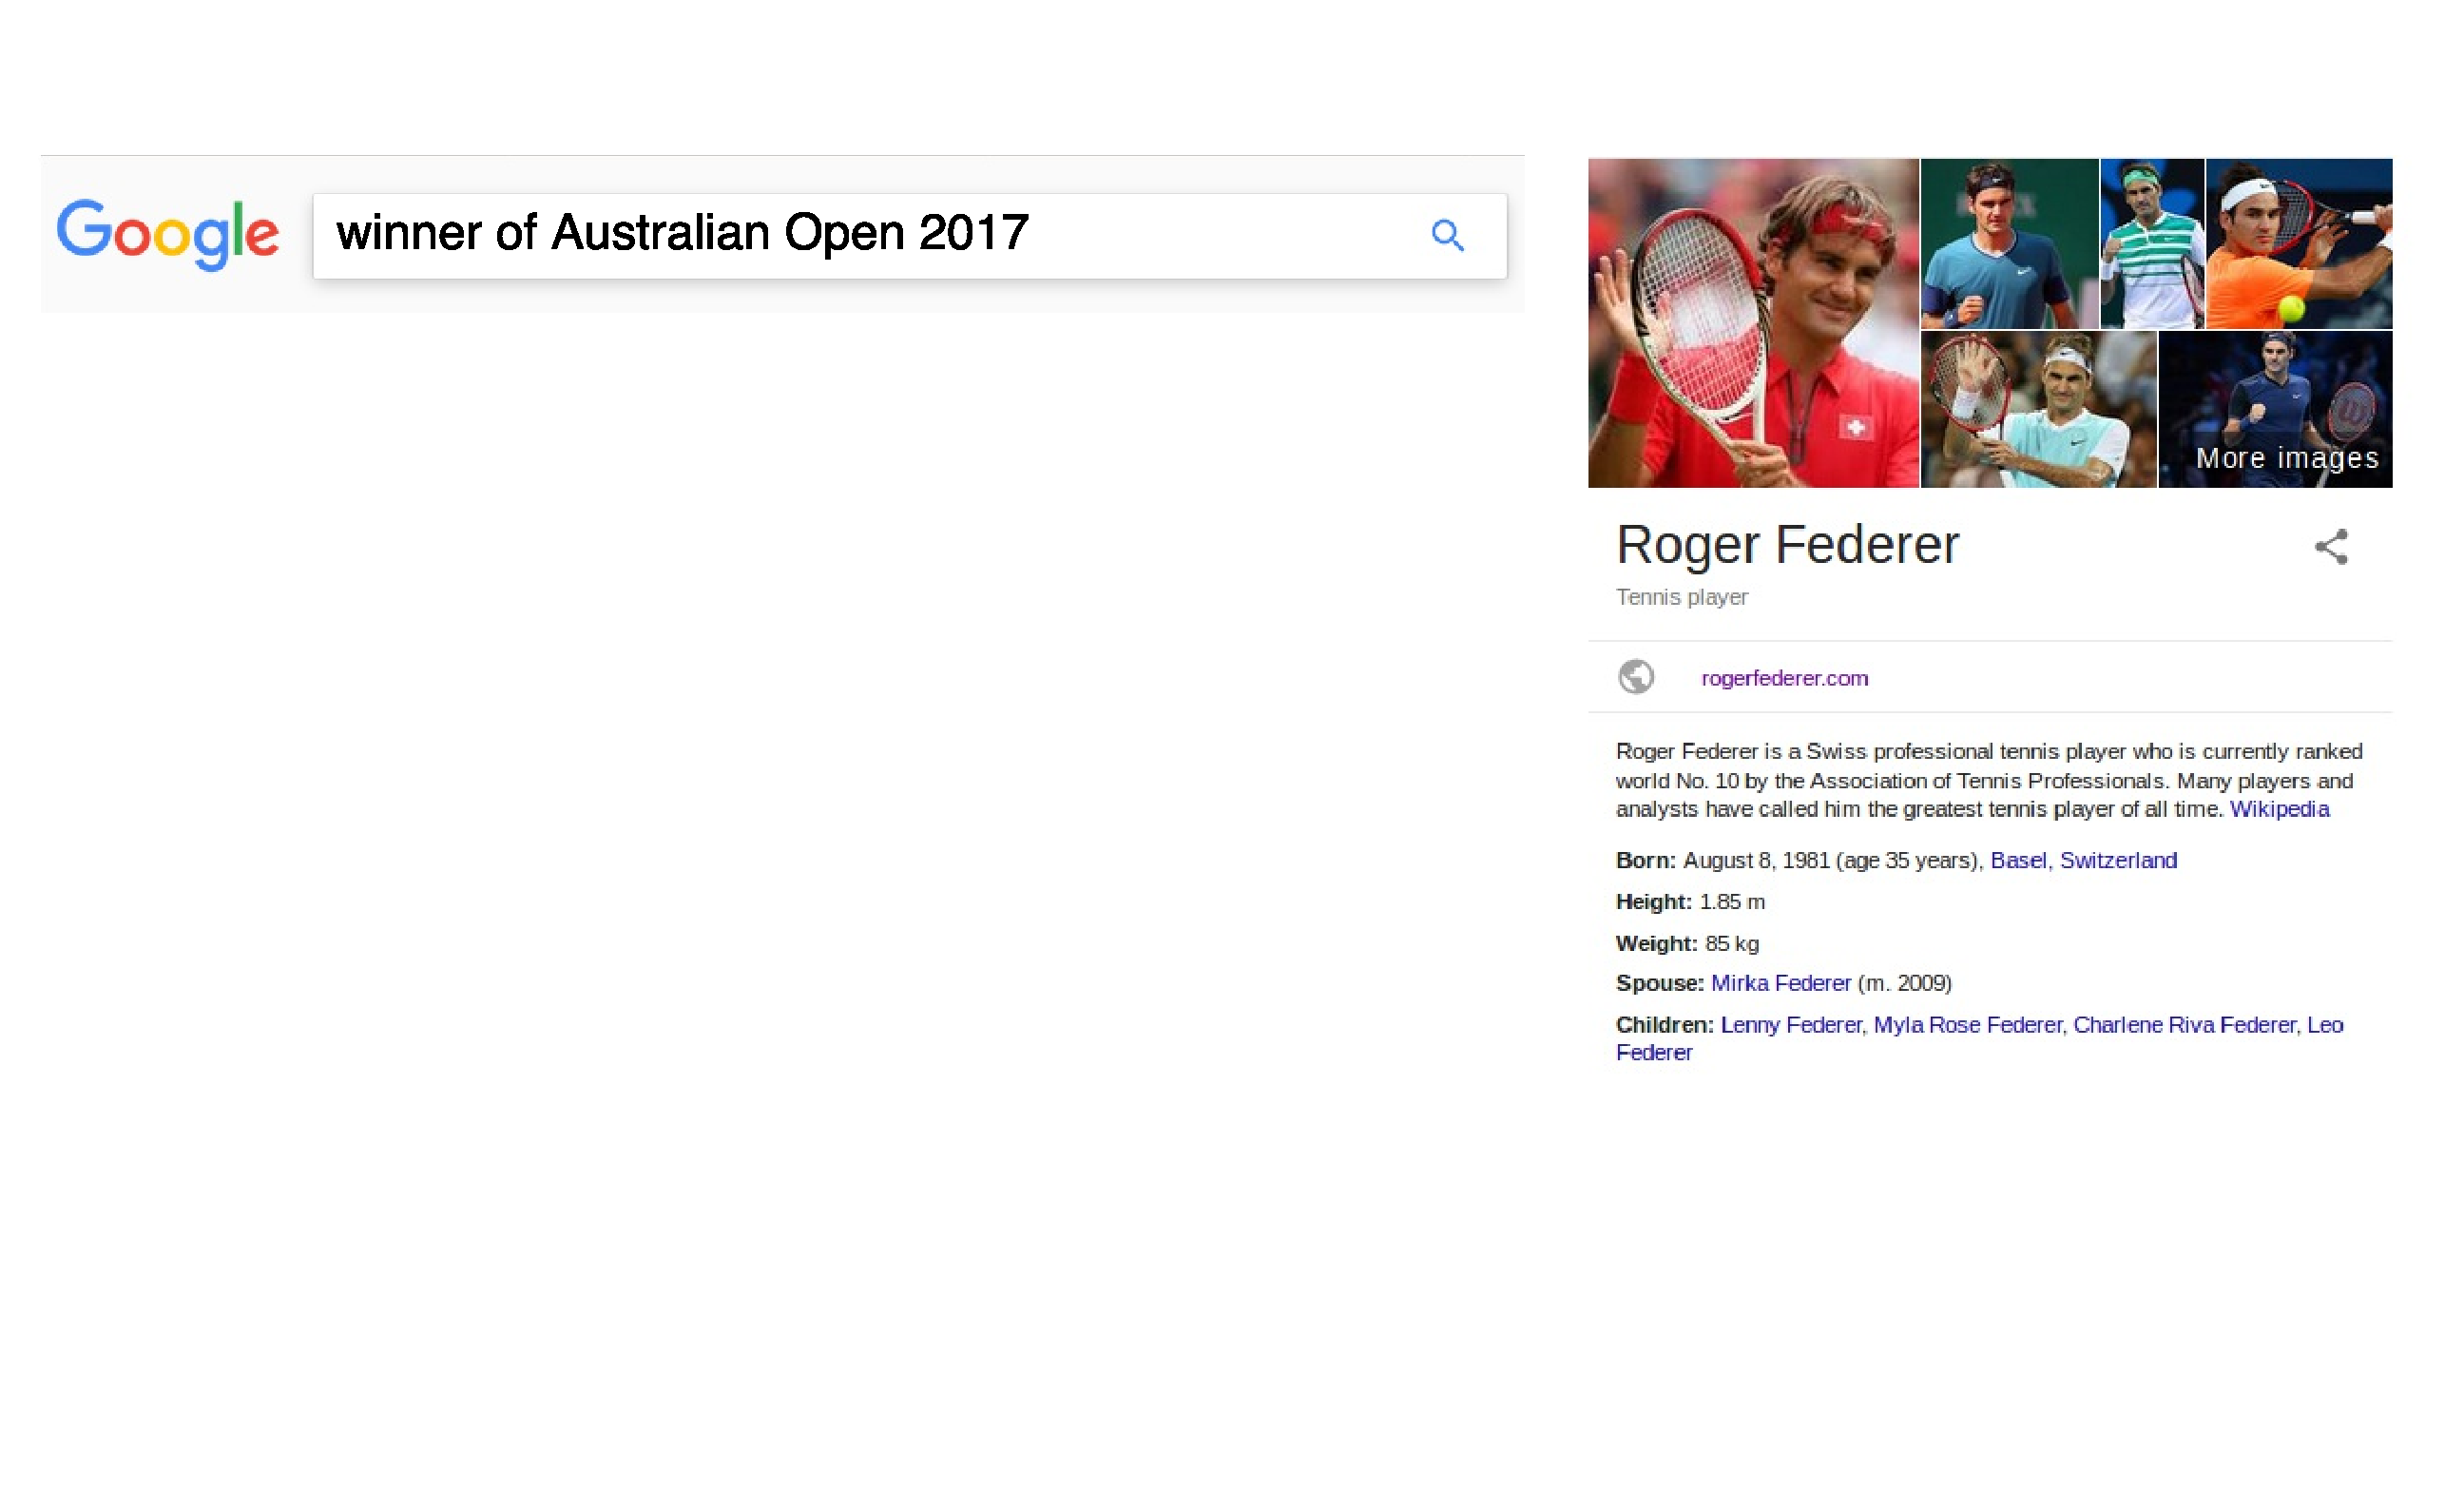
\includegraphics[width=1.1\textwidth]{semsearch1}}
% \end{picture}
% }}


% \end{frame}


% \begin{frame}\frametitle{Knowledge Graphs}
%  \alt<2->{


% \begin{picture}(0.5,0.5)
% \put(217,-130){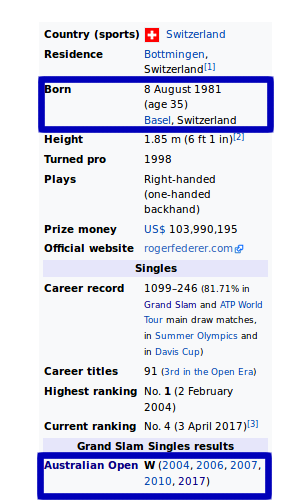
\includegraphics[width=.41\textwidth]{rf_wiki2}}
% \end{picture}
% \begin{picture}(0.5,0.5)
% \put(-5,-120){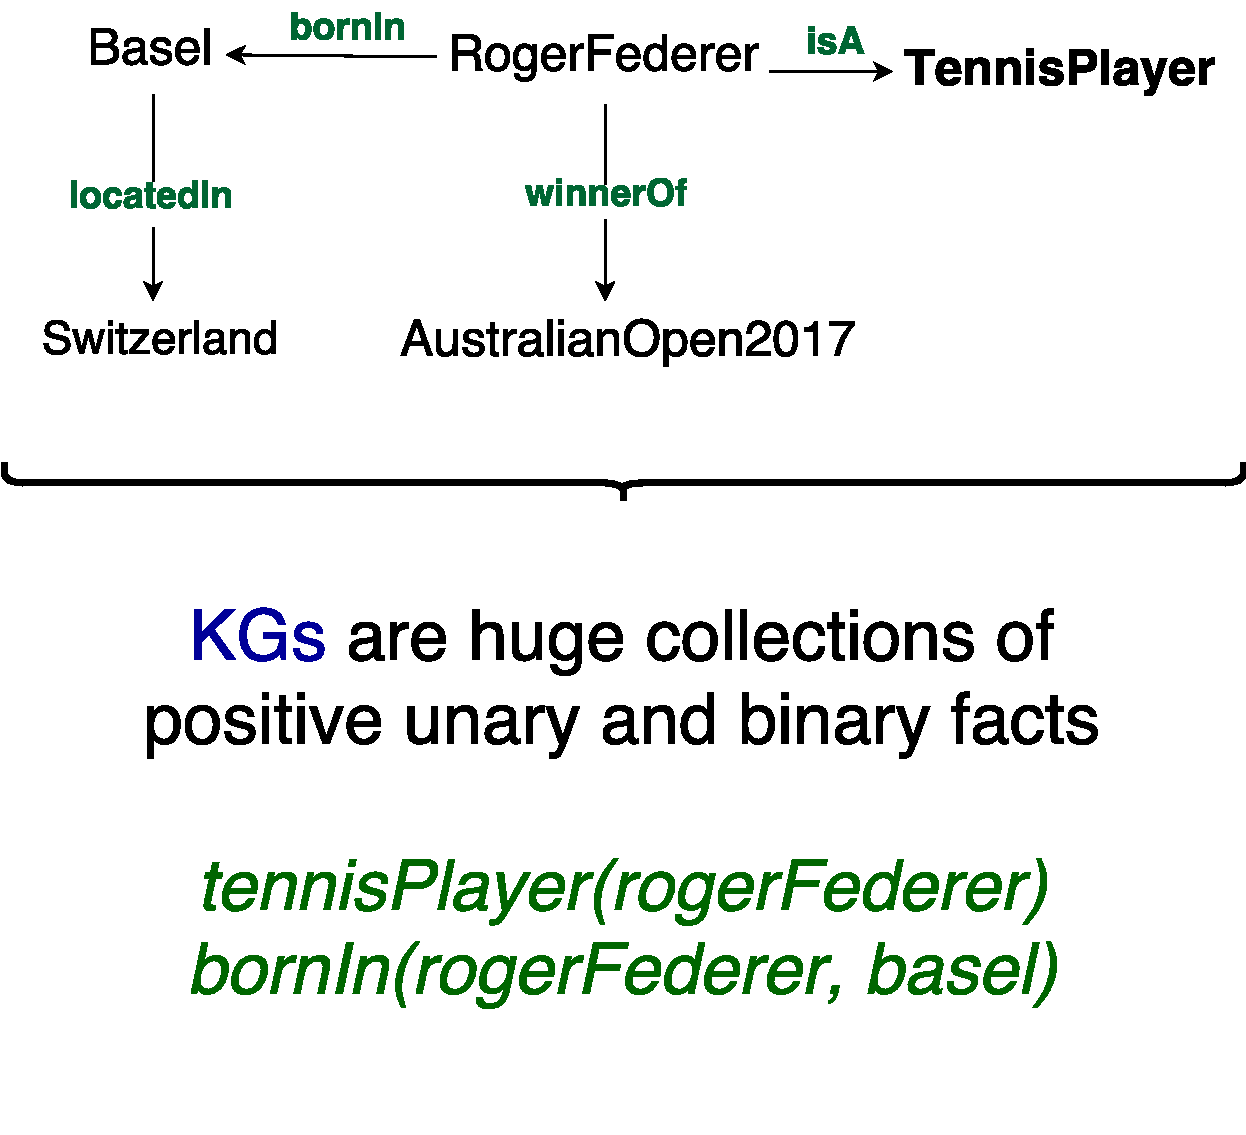
\includegraphics[width=.65\textwidth]{kg_general1}}
% \end{picture}


% }{\begin{picture}(0.5,0.5)
% \put(23,-135){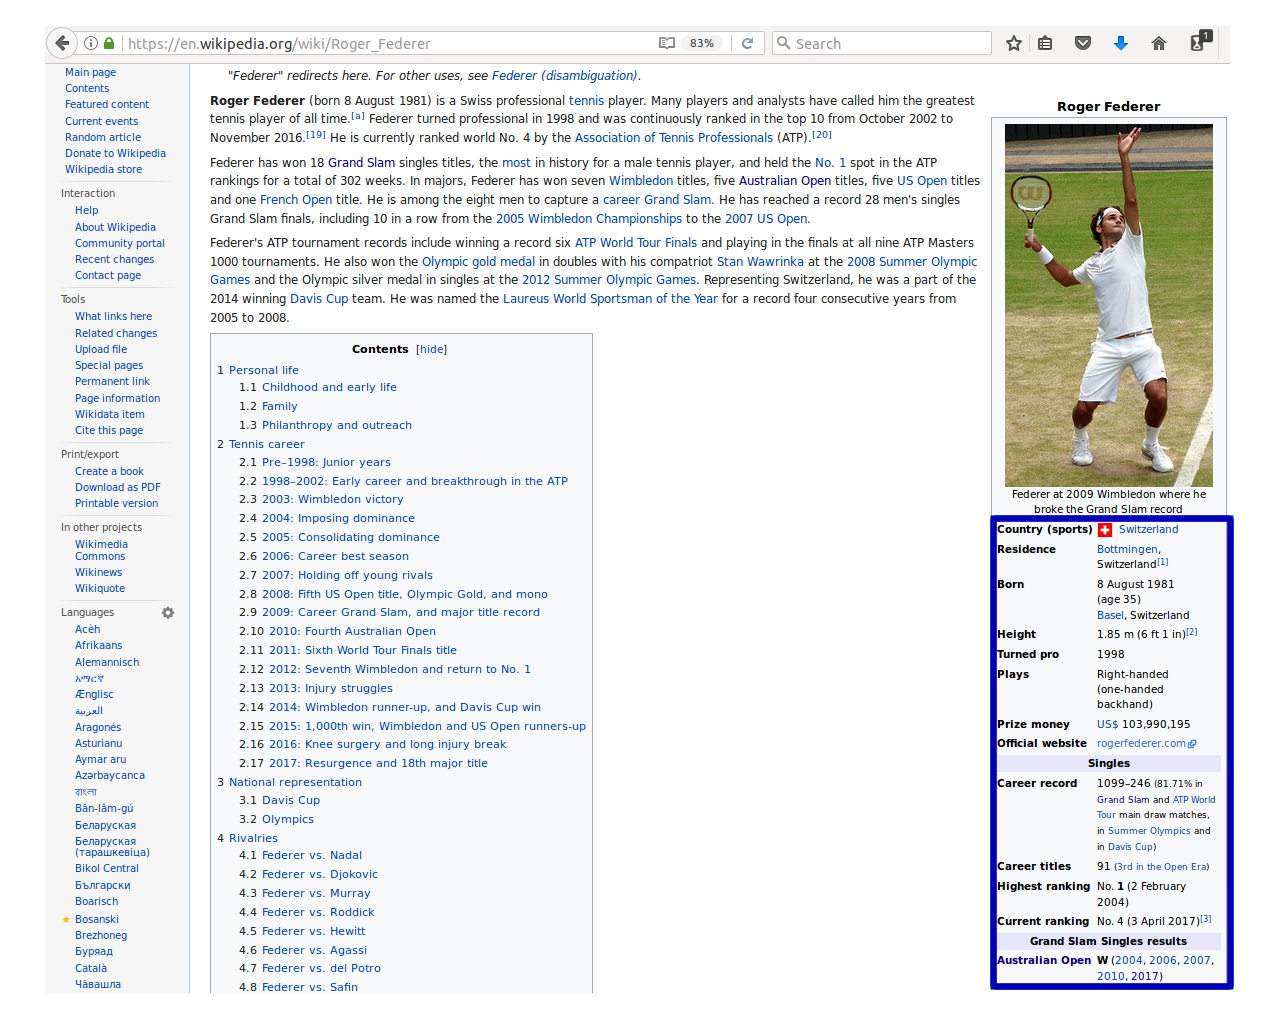
\includegraphics[width=.85\textwidth]{rf_wiki}}
% \end{picture}}
% \end{frame}

% \begin{frame}\frametitle{Problem: Inconsistency}
% %\alt<2>{
% 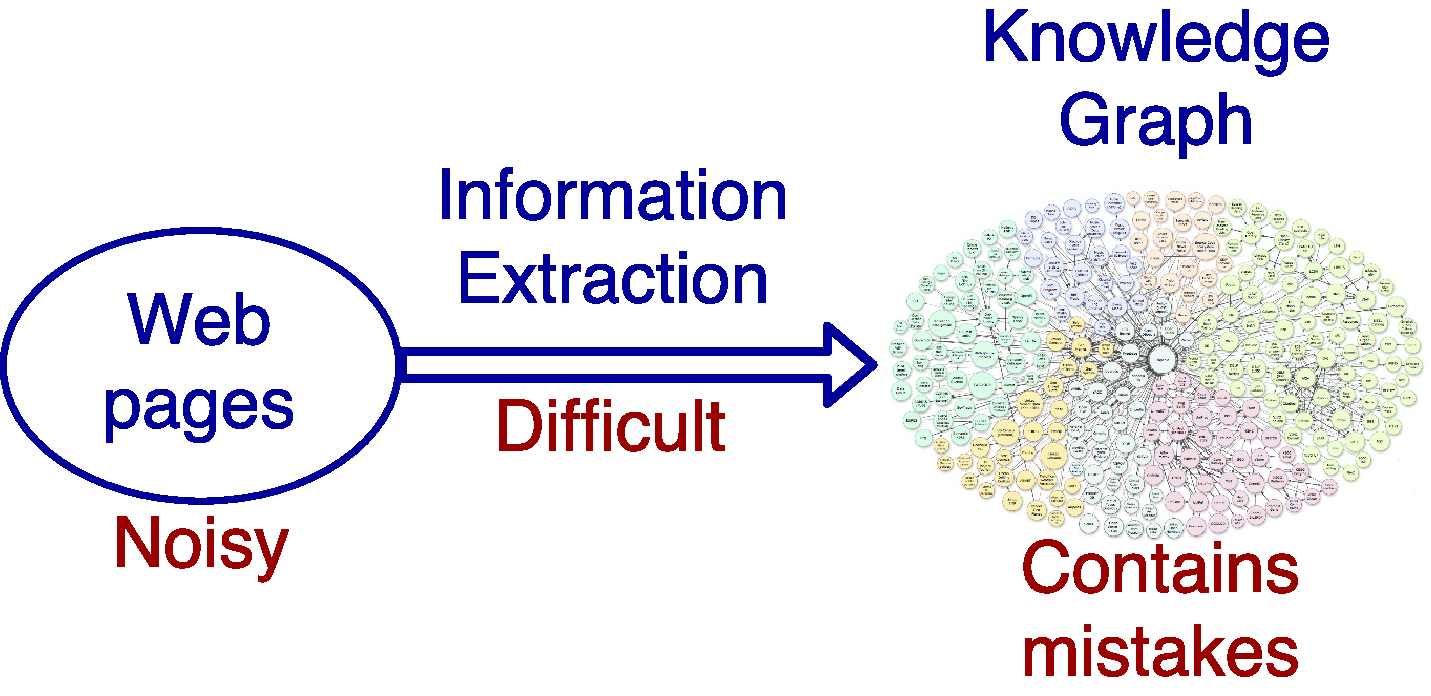
\includegraphics[width=1\textwidth]{kg_problem1}
% %}{\includegraphics[width=1\textwidth]{kg_er}}

% \end{frame}


% \begin{frame}\frametitle{Problem: Incompleteness}
% \bigskip

% Google KG \alert{misses} Roger's living place, but contains his wife's Mirka's.. 
% \bigskip

% \begin{center}
% 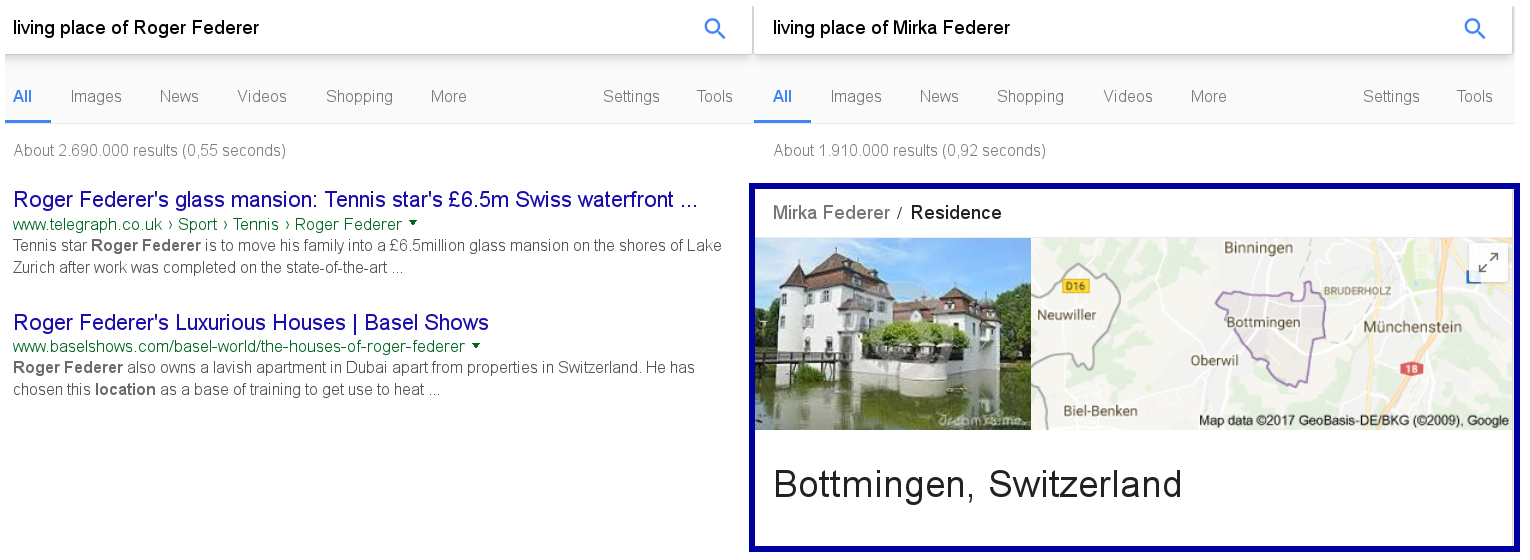
\includegraphics[width=1.02\textwidth]{kg_problem2}
% \end{center}
% \end{frame}

% % \begin{frame}\frametitle{Inconsistency and Incompleteness in KGs}
% % \bigskip

% % \alt<2>{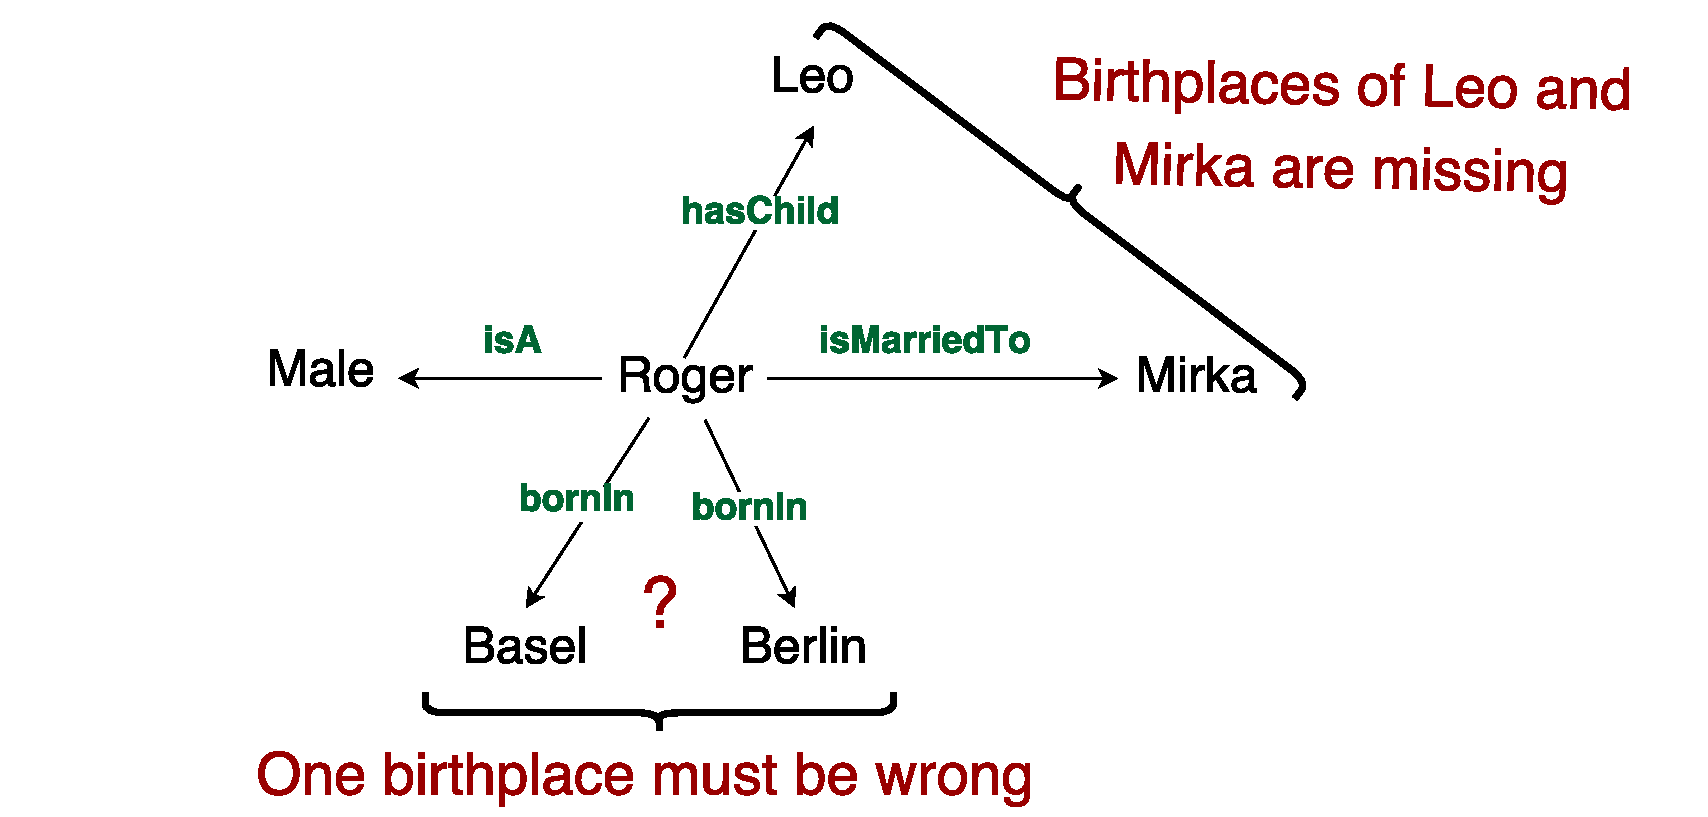
\includegraphics[width=1\textwidth]{kg_inc2}}{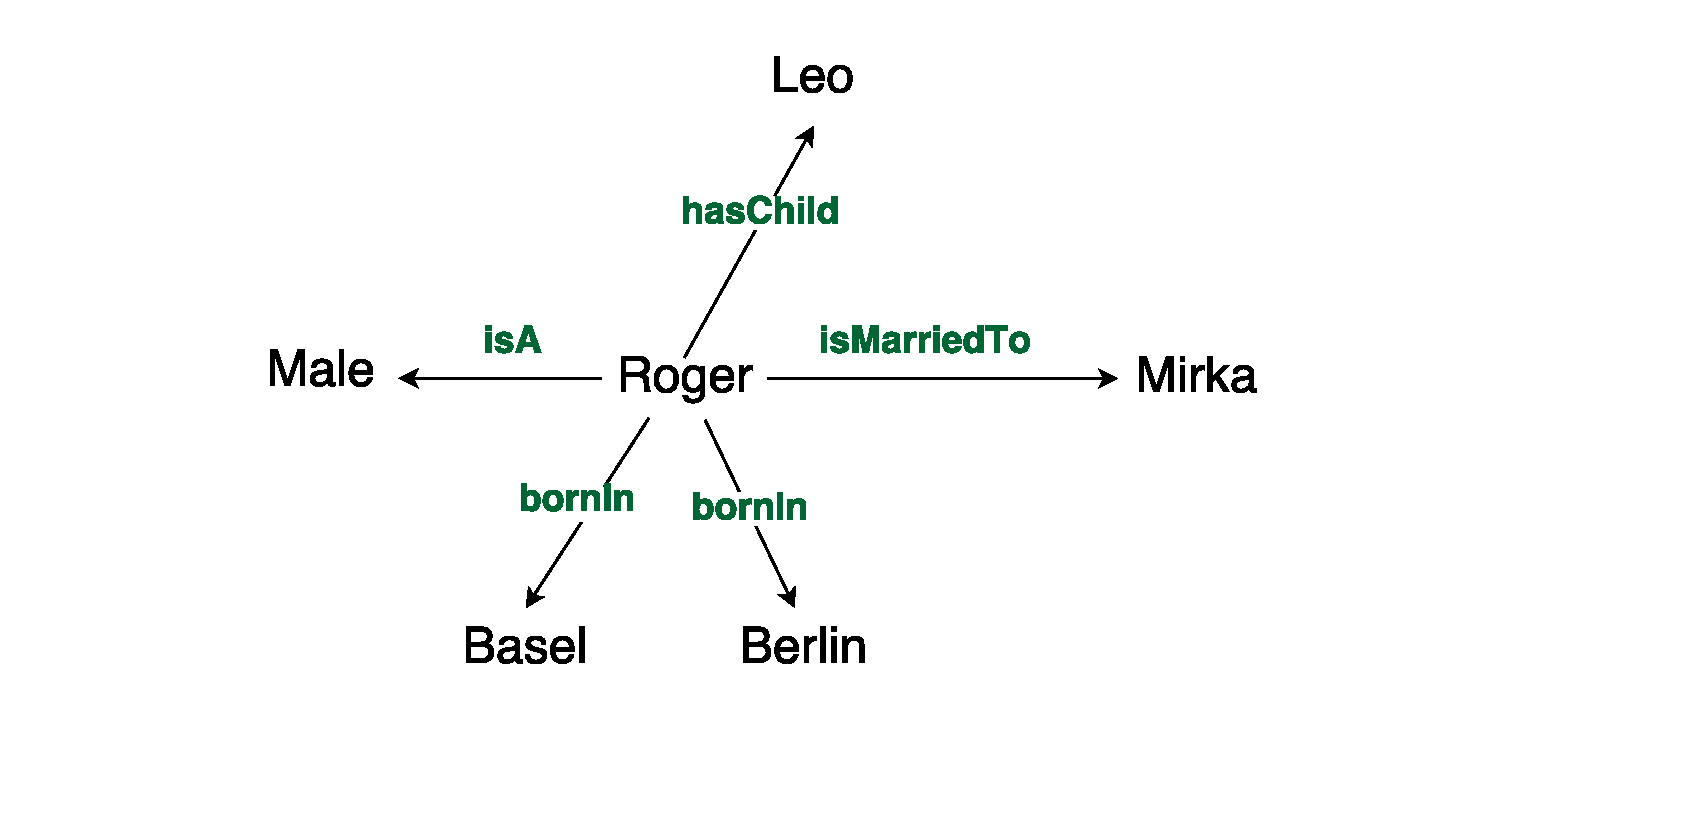
\includegraphics[width=1\textwidth]{kg_inc1}}
% % \end{frame}


% \begin{frame}\frametitle{Motivation}
% \begin{beamerboxesrounded}[upper=uppercolred,lower=lowercolred,shadow=true]{\textbf{\alert{Important problems}} of KGs:}

%  \medskip
%  \begin{itemize}
%  \item[\alert{\circled{1}}] \alert{Inconsistency}
%  \medskip

%  \item[\alert{\circled{2}}] \alert{Incompleteness}
%  \end{itemize}
%  \end{beamerboxesrounded}
% \bigskip
% \bigskip
% \bigskip

% \begin{beamerboxesrounded}[upper=uppercolblue,lower=lowercolblue,shadow=true]{\textbf{\bl{In this talk: }} Reasoning on top of KGs to address these issues}

%  \medskip
%  \begin{itemize}
%  \item[\circledbl{1}] \bl{Deduction}: detecting and \bl{repairing inconsistencies} %and \bl{inconsistency repair}
%  \medskip

%  \item[\circledbl{2}] \bl{Induction}: learning common-sense rules and \bl{completing} KGs
%  \end{itemize}
%  \end{beamerboxesrounded}
% \end{frame}


% %%%%%%%%%%%%%%%%%%%%%%%%%%%%%%%%%%%%%%%%%%%%%%%%%%%%%%%%%%%%%%%%%%%

% %\makeoverview
% \section{Ontologies and Rules}

% \begin{frame}\frametitle{Overview}
% \begin{itemize}
% \item[$\checkmark$] \bl{Motivation}
% \bigskip

% \item[] \textbf{\bl{Ontologies and Rules}}
% \bigskip

% \item[] \bl{Inconsistencies in DL-programs}
% \bigskip

% \item[] \bl{Nonmonotonic Rule Mining}
% \bigskip

% \item[] \bl{Further and Future Work}
% \end{itemize}
% \end{frame}


% %%%%%%%%%%%%%%%%%%%%%%%%%%%%%%%%%%%%%%%%%%%%%%%%%%%%%%%%%%%%%%%%%%%


% \begin{frame}
% \frametitle{History of Knowledge Representation}
% \small{\begin{itemize}
% \item \textbf{\bl{1950's:}} \bl{First Order Logic (FOL)} for KR (\alert{undecidable})\\
% (e.g. \cite{M59})
% \bigskip

% \item \textbf{\bl{1970's:}} \bl{Network-shaped structures} for KR (\alert{no formal semantics})\\
% (e.g. semantic networks \cite{semnet}, frames \cite{frames})
% \bigskip

% \item \textbf{\bl{1979:}} Encoding of \bl{network-shaped structures} into \bl{FOL} \cite{hayes79}
% \bigskip

% \item \textbf{\bl{1980's:}} \textcolor{blue}{Description Logics (DL)} for KR
% \begin{itemize}
% \item \bl{Decidable fragments} of \bl{FOL}
% \item Theories encoded in DLs are called \bl{ontologies}
% \item Many DLs with different expressiveness and computational features
% \item Particularly suited for \bl{conceptual reasoning}
% \end{itemize}
%  \end{itemize}}
% \end{frame}



% \begin{frame}
% \frametitle{Description Logic Ontologies}
% \textbf{\bl{Open World Assumption (OWA)}}: what is not derived is \bl{unknown}

%  \alt<2>{\begin{picture}(0.5,0.5)
%    \put(50,-136){\includegraphics[width=0.7\textwidth]{dl1}}
%   \end{picture}}{\begin{picture}(0.5,0.5)
%    \put(50,-136){\includegraphics[width=0.7\textwidth]{dl0}}
%   \end{picture}}
% \bigskip
% \bigskip
% \bigskip
% \bigskip
% \bigskip
% \bigskip
% \bigskip
% \bigskip
% \bigskip
% \bigskip
% \bigskip
% \bigskip
% \bigskip

% \begin{beamerboxesrounded}[upper=uppercolgreen,lower=lowercolgreen,shadow=true]{}
% \small{

% \textbf{Inclusions:} \gr{$\mi{Female \sqsubseteq \neg Male{,}hasSister \sqsubseteq hasSibling{,}hasBrother \sqsubseteq hasSibling}$}
% \smallskip
% \pause 

% \vspace{-.2cm}
% \textbf{Complex axioms:} \gr{\alt<2>{$\mi{Uncle \equiv Male \sqcap \exists hasSibling.\exists hasChild}$}{$\mi{\forall X\exists Y\,Z(Female(X) \wedge hasSibling(X,Y)\wedge hasChild(Y,Z))}$}}
% }
% \end{beamerboxesrounded}


% \end{frame}



% \begin{frame}\frametitle{What can not be said in DLs?}
% \begin{itemize}


% \item \bl{Exceptions} from theories (due to \bl{monotonicity})\\
% \end{itemize}
% \begin{center}
% \begin{columns}
% \begin{column}{.39\textwidth}
%  \uncover<2-4>{

%  $\gr{\mi{WithBeard \sqsubseteq Male}}$\\
%  $\gr{\mi{Female \sqsubseteq \neg Male}}$\\
%  $\gr{\mi{WithBeard(c)}}$\\
% }
%  \uncover<4->{\bl{$\mi{Female(c)}$\\}}
%  \uncover<2-4>{------------------------------------\\}
%  \uncover<3->{\gr{$\mi{Male(c)}$\\}}
%  \uncover<4->{\bl{$\neg \mi{Male(c)}$}\\}
% \end{column}
% \begin{column}{.39\textwidth}
%  \uncover<2-4>{

%  \emph{People with beards are male}\\
%  \emph{Female are not male}\\
%  \emph{C has a beard}\\
%  }
%  \uncover<4->{\emph{C is female}\\}
%  \uncover<2-4>{------------------------------------\\}
%  \uncover<3->{\emph{C is male}\\}
%  \uncover<4>{\emph{C is not male}\\}
% \end{column}
% \end{columns}
% \end{center}
% \uncover<4>{\begin{picture}(0.5,0.5)
%  \put(95,-10){\includegraphics[width=.25\textwidth]{malefemale}}
%  \end{picture}
% \bigskip

% \begin{center}\bl{Monotonicity:} the more we add, the more we get!\end{center}

% }
% \end{frame}


% \begin{frame}
%   \frametitle{History of Knowledge Representation}
% \bigskip
% \bigskip

% \begin{itemize}
% \item \textbf{\bl{1970's:}} \bl{Logic programming} \\(e.g. Prolog)
% \bigskip
% \bigskip

% \item \textbf{\bl{1980's:}} \bl{Nonmonotonic logics}\\ (e.g. circumscription \cite{DBLP:journals/ai/McCarthy80}, default logic \cite{DBLP:journals/ai/Reiter80})
% \bigskip
% \bigskip

% \item \bl{\textbf{1988:}} \bl{Nonmonotonic rules} under \bl{answer set semantics} (ASP) \\\cite{GL1988}
% \begin{itemize}
% \item \normalsize{Logic programs with \bl{model-based} semantics}
% \item \normalsize{\bl{Disjunctive datalog} with \bl{default negation} $\bl{\mi{not}}$}
% \end{itemize}

% \end{itemize}

% \end{frame}

% \begin{frame}\frametitle{Not is not $\neg$!}
%  \begin{beamerboxesrounded}[upper=uppercolgreen,lower=lowercolgreen,shadow=true]{\normalsize{\textbf{Default negation}} \large{\bl{$\naf$}} 
%    }
% \medskip

% At a rail road crossing cross the road if \textbf{no train is known} to approach\medskip

% \gr{$\mi{walk}\leftarrow \mi{at(X), crossing(X), \text{\emph{\textbf{not}} } train\_approaches(X)}$}

% \end{beamerboxesrounded}
% \bigskip
% \bigskip
% \bigskip

%  \begin{beamerboxesrounded}[upper=uppercolgreen,lower=lowercolgreen,shadow=true]{\normalsize{\textbf{Classical negation}}  \large{\bl{$\neg$}} 
%    }
% \medskip

% At a rail road crossing cross the road if \textbf{no train} approaches\medskip

% \gr{$\mi{walk}\leftarrow \mi{at(X), crossing(X), \neg train\_approaches(X)}$}
% \end{beamerboxesrounded}
% \end{frame}

% \begin{frame}\frametitle{Nonmonotonic Rules}
% \bigskip

% \bl{\textbf{Closed World Assumption (CWA):} } what is not derived is \bl{false}
% \bigskip
% \bigskip

% \small{ \bl{\textbf{Rule:} }
% $\underbrace{a_1 \lor \dotsc \lor a_k}_{\Large{\bl{\text{head}}}}\; \leftarrow\; \underbrace{b_1,\, \dotsc,\, b_m,\,\bl{not} \,b_{m+1},\,\dotsc,\,\bl{not} \,b_n}_{\bl{\text{body}}} $

% }
% \bigskip
% \bigskip

% \small{\bl{\textbf{Informal semantics:}} } If $b_1,\dotsc, b_{m}$ are true and \bl{none} of $b_{m+1},\dotsc,b_n$ is \bl{known}, \phantom{\textbf{Informal semantics:\;\;\;}}then at least one among $a_1,\dotsc, a_k$ must be true\bigskip
% \bigskip
% \bigskip

% \begin{beamerboxesrounded}[upper=uppercolgreen,lower=lowercolgreen,shadow=true]{}
% \small{
% \textbf{Default negation}: unless a child is adopted one of his parents must be female\medskip

% \gr{$\mi{female(Y)\lor female(Z)\leftarrow hasParent(X,Y),hasParent(X,Z),} \\
% \phantom{\mi{female(Y)\lor female(Z)\leftarrow}}\mi{Y \neq Z, \naf\,adopted(X)}$}
% \bigskip

% \textbf{Constraint:} ensure that no one is a parent of himself\medskip

% \gr{$ \bot \leftarrow \mi{parent(X,Y),parent(Y,X)}$}
% }

% \end{beamerboxesrounded}
% \bigskip

% \end{frame}


% %%%%%%%%%%%%%%%%%%%%%%%%%%%%%%%%%%%%%%%%%%%%%%%%%%%%%%%%%%%%%%%%%%%


% \begin{frame}
% \frametitle{Answer Set Programs}
% \begin{itemize}
% \item[]\uncover<1->{\bl{Evaluation} of ASP programs is model-based }%\footnote{unlike in prolog, which is based on theorem proving}}%\uncover<3->{, it consists of 2 steps:}
% \begin{itemize}
% \uncover<2->{\item[1.]\bl{Grounding}: substitute all \bl{variables with constants} in all possible ways }
% \uncover<4->{\item[2.]\bl{Solving}: compute a \bl{minimal model (answer set) $I$} satisfying all rules}
% \end{itemize}
% \end{itemize}
% \bigskip

% \begin{beamerboxesrounded}[upper=uppercolgreen,lower=lowercolgreen,shadow=true]{\textbf{Answer set program (ASP)} is a set of nonmonotonic rules}
% \bigskip

% $\gr{
%       \begin{array}{l@{\qquad}}
%          \mbox{(1) }\mi{hasParent(john,pat)}\;\;\; \mbox{(2) }\mi{hasParent(john,alex)}\;\;\;\mbox{(3) }\mi{male(alex)}\\[0.35ex]
%          \mbox{(4) }\mi{female(\alt<3->{\mi{pat}}{\bl{Y}})} \leftarrow \alt<3->{\mi{hasParent(john,pat)}}{\mi{hasParent(\bl{X,Y})}},\mi{hasParent(\alt<3->{john,alex}{\bl{X,Z}}),}\\
%          \phantom{\mbox{(4) }\mi{female(\alt<3->{pat}{\bl{Y}})\,} \leftarrow }\only<1,2>{\bl{Y\neq Z},} \mi{male(\alt<3->{alex}{\bl{Z}})},\naf\ \mi{adopted(\alt<3->{\mi{john}}{\bl{X}})} \uncover<5->{\\[0.35ex]\bl{\mbox{(5) }\mi{adopted(john)}}}
%       \end{array}
%     }$
% \medskip

% \uncover<5->{\small{$\phantom{\mi{I{=}\{\mi{hasParent(john,pat),hasParent(john,alex),male(alex)}}}\bl{\mi{adopted(john)}}$}}
% \uncover<4->{
% \small{$\gr{\mi{I{=}\{\mi{hasParent(john,pat),hasParent(john,alex),male(alex)},\alt<5>{\cancel{\mi{female(pat)}}}{\mi{female(pat)}}\}}}$}

% \uncover<4>{\medskip

% \bl{CWA:} \gr{$\mi{adopted(john)}$} can not be derived, thus it is false}}

% \end{beamerboxesrounded}


% \begin{center}\visible<5>{\bl{Nonmonotonicity}: adding facts might lead to loss of consequences!}\end{center}
% \end{frame}


%  \begin{frame}\frametitle{Combining Ontologies and Rules}
%  \begin{picture}(0.5,0.5)
% \alt<2>{\put(50,-130){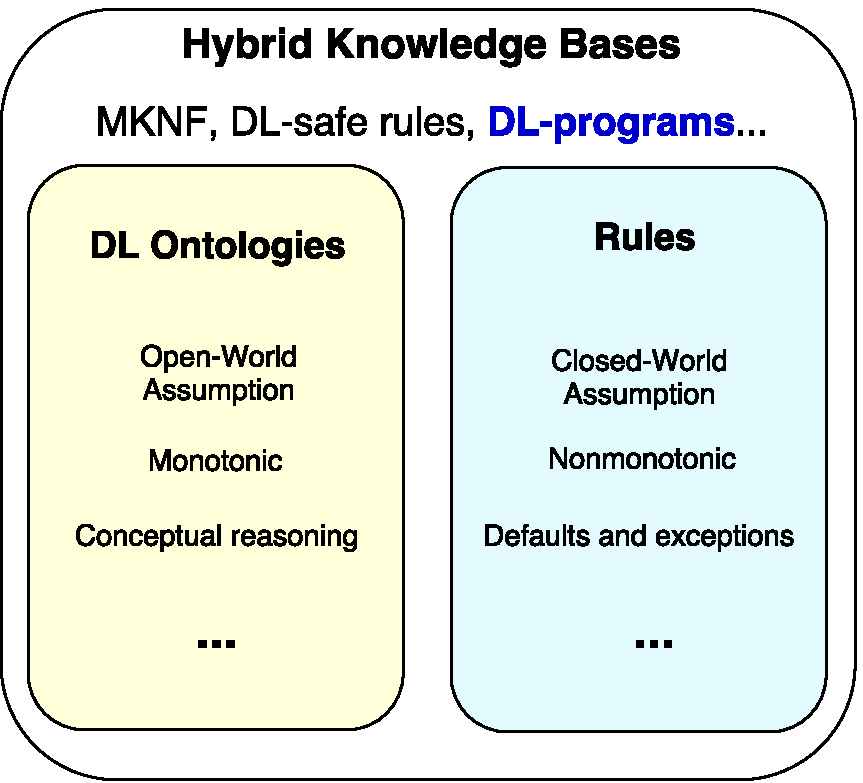
\includegraphics[width=0.7\textwidth]{dlvsrules}}}{\put(50,-130){\includegraphics[width=0.7\textwidth]{dlvsrules0}}}
%  \end{picture}

%  \end{frame}

% \section{Inconsistencies in DL-programs}

% \begin{frame}\frametitle{Overview}
% \begin{itemize}
% \item[$\checkmark$] \bl{Motivation}
% \bigskip

% \item[$\checkmark$] \bl{Ontologies and Rules}
% \bigskip

% \item[] \textbf{\bl{Inconsistencies in DL-programs}}
% \bigskip


% \item[] \bl{Nonmonotonic Rule Mining}
% \bigskip

% \item[] \bl{Further and Future Work}
% \end{itemize}

% \begin{picture}(0.5,0.5)
% \put(200,65){\includegraphics[width=0.11\textwidth]{eiter}}
% \put(204,55){\text{\footnotesize{T. Eiter}}}
% \end{picture}

% \begin{picture}(0.5,0.5)
% \put(265,78){\includegraphics[width=0.095\textwidth]{fink}}
% \put(267,68){\text{\footnotesize{M. Fink}}}
% \end{picture}
% \end{frame}



% \begin{frame}\frametitle{DL-programs}
% \bl{DL-programs:} loose coupling of \bl{ontologies} and \bl{rules} \cite{EIL08}
% \bigskip
% \bigskip
% \bigskip
% \bigskip
% \bigskip
% \bigskip
% \bigskip
% \bigskip
% \bigskip
% \bigskip
% \bigskip
% \bigskip
% \bigskip
% \bigskip

% \begin{picture}(0.5,0.5)
% \put(80,-25){\includegraphics[width=0.53\textwidth]{dlp}}
% \end{picture}
% \end{frame}


% \begin{frame}\frametitle{\alt<15->{DL-program Repair}{\alt<14>{Inconsistent DL-program}{DL-program}}}
% \bigskip

% \small{
% \begin{beamerboxesrounded}[upper=uppercolgreen,lower=lowercolgreen,shadow=true]{\centerline{DL ontology}}
% \vspace{-.1cm}
%  \begin{columns}
%  \begin{column}{.38\textwidth}
% \begin{beamerboxesrounded}[upper=uppercolgreen,lower=lowercolgreen,shadow=true]{\centerline{Logical part}}
% \vspace{-.2cm}
% \gr{\begin{center}\small{$%O{=}\left\{
% \begin{array}{@{\,}l@{}}
%  \mbox{(1) }\mathit{Child \sqsubseteq \exists hasParent} \\[0.25ex]
%  \mbox{(2) }\mathit{Female \sqsubseteq \neg Male}  \\[0.25ex] 
% \mbox{(3) } \mathit{Adopted \sqsubseteq Child} \\[0.25ex]
%  \end{array}
% %\right\}
% $}
% \end{center}}
%  \end{beamerboxesrounded}
%  \end{column}
%  \begin{column}{.49\textwidth}
% \begin{beamerboxesrounded}[upper=uppercolgreen,lower=lowercolgreen,shadow=true]{\centerline{Data part (KG)}}
% \vspace{-.2cm}
% \gr{\begin{center}\small{$%O{=}\left\{
% \begin{array}{@{\,}l@{\,}l@{}}
%  \alt<16>{\bl{\mbox{(4) }\cancel{\mathit{Male(pat)}}\,\,\mathit{Female(pat)}}}{\alt<7>{\bl{\mbox{(4) }\mathit{Male(pat)}}}{\mbox{(4) }\mathit{Male(pat)}}}& \alt<15>{\bl{\mi{Female(alex)}}}{\alt<7>{\mi{Male(tim)}}{\uncover<6,7>{\bl{\mi{Male(tim)}}}}}\\[0.25ex]
%  \mbox{(5) }\mathit{Male(john)}&  \\[0.25ex] 
% \alt<17>{}{\alt<3>{\bl{\mbox{(6) }\mi{hasParent(john,pat)}}}{\mbox{(6) } \mathit{hasParent(john,pat)}}}& \\[0.25ex]
%  \end{array}
% %\right\}
% $}
% \end{center}}
%  \end{beamerboxesrounded}
%  \end{column}
% \end{columns}
% \end{beamerboxesrounded}
% }
% \bigskip

%  \begin{beamerboxesrounded}[upper=uppercolgreen,lower=lowercolgreen,shadow=true]{\centerline{Rules}}
%  \vspace{-.1cm}
% \gr{\small{\begin{center}
% $\begin{array}{@{\,}l@{~\,}}
% \alt<11>{\bl{ \mbox{(7) }\mi{isChildOf(john,alex)}}}{ \mbox{(7) }\mi{isChildOf(john,alex)}}\;\;\;\;\;\;\alt<6>{\bl{(8)\; \mi{boy(tim)}}}{(8)\; \mi{boy(tim)}}\\[0.35ex]
%  \mbox{(9) }\mi{hasFather}(john,pat) \leftarrow \alt<2->{\dlatom{}{\alt<3>{\bl{\mi{hasParent}}}{\mi{hasParent}}}{\alt<3>{\bl{\mi{john,pat}}}{\mi{john,pat}}}\only<3-8>{\;\;\bl{\checkmark}}}{\call}, \alt<4->{\\
% \phantom{\mbox{(9) }\mi{hasfather}(john,pat) \leftarrow}\;\; \dlatom{\alt<5,6>{\bl{\mi{Male} \uplus \mi{boy}}}{\mi{Male} \uplus \mi{boy}}}{\alt<7>{\bl{\mi{Male}}}{\mi{Male}}}{\alt<7>{\bl{\mi{pat}}}{\mi{pat}}}\only<7-8>{\;\;\bl{\checkmark}}}{\call}\\[0.35ex]
% \alt<14>{\alert{\mbox{(10) }\bot \leftarrow \mi{hasFather(john,pat),isChildOf(john,alex)},}\\
% \phantom{\mbox{(10) }\bot \leftarrow }\; \alert{\naf\dlatom{}{\mi{Adopted}}{john},}\\
% \phantom{\mbox{(10) }\bot \leftarrow }\; \alert{\naf\dlatom{\mi{Child}\uplus\mi{boy}}{\neg \mi{Male}}{\mi{alex}}}
% }{\alt<9->{\mbox{(10) }\bot \leftarrow \alt<10-14>{\bl{\mi{hasFather(john,pat)}}}{\mi{hasFather(john,pat)}},\alt<11-14>{\bl{\mi{isChildOf(john,alex)}}}{\mi{isChildOf(john,alex)}},\\
% \phantom{\mbox{(10) }\bot \leftarrow }\; \alt<12-14>{\bl{\naf\dlatom{}{\mi{Adopted}}{john}}}{\naf\dlatom{}{\mi{Adopted}}{john}},\\
% \phantom{\mbox{(10) }\bot \leftarrow }\; \alt<13-14>{\bl{\naf\dlatom{\mi{Child}\uplus\mi{boy}}{\neg \mi{Male}}{alex}}}{\naf\dlatom{\mi{Child}\uplus\mi{boy}}{\neg \mi{Male}}{alex}}\\}{}}
% \end{array}$%
%  \end{center}}}
%  \end{beamerboxesrounded}
%  \medskip

% \alt<15,16,17>{\bl{Repair answer set: }\gr{$\mi{I=\{isChildOf(john,alex),boy(tim)}\only<15>{\mi{,hasFather(john,pat)}}\}$}}{\alt<14>{\alert{\textbf{Inconsistent DL-program}: no answer sets!}}{\uncover<8>{\small{\bl{Answer set:} \gr{$\mi{I=\{isChildOf(john,alex),boy(tim),hasFather(john,pat)\}}$}}}}}



% \end{frame}


% \begin{frame}
% \frametitle{Inconsistency Handling in DL-programs}
% \bigskip

% \small{\bl{\textbf{Goal:}} develop techniques for handling inconsistencies in DL-programs}\\
% \small{\bl{\textbf{Approach:}} repair ontology data part (KG) to regain consistency}
% \smallskip

% \begin{center}
% 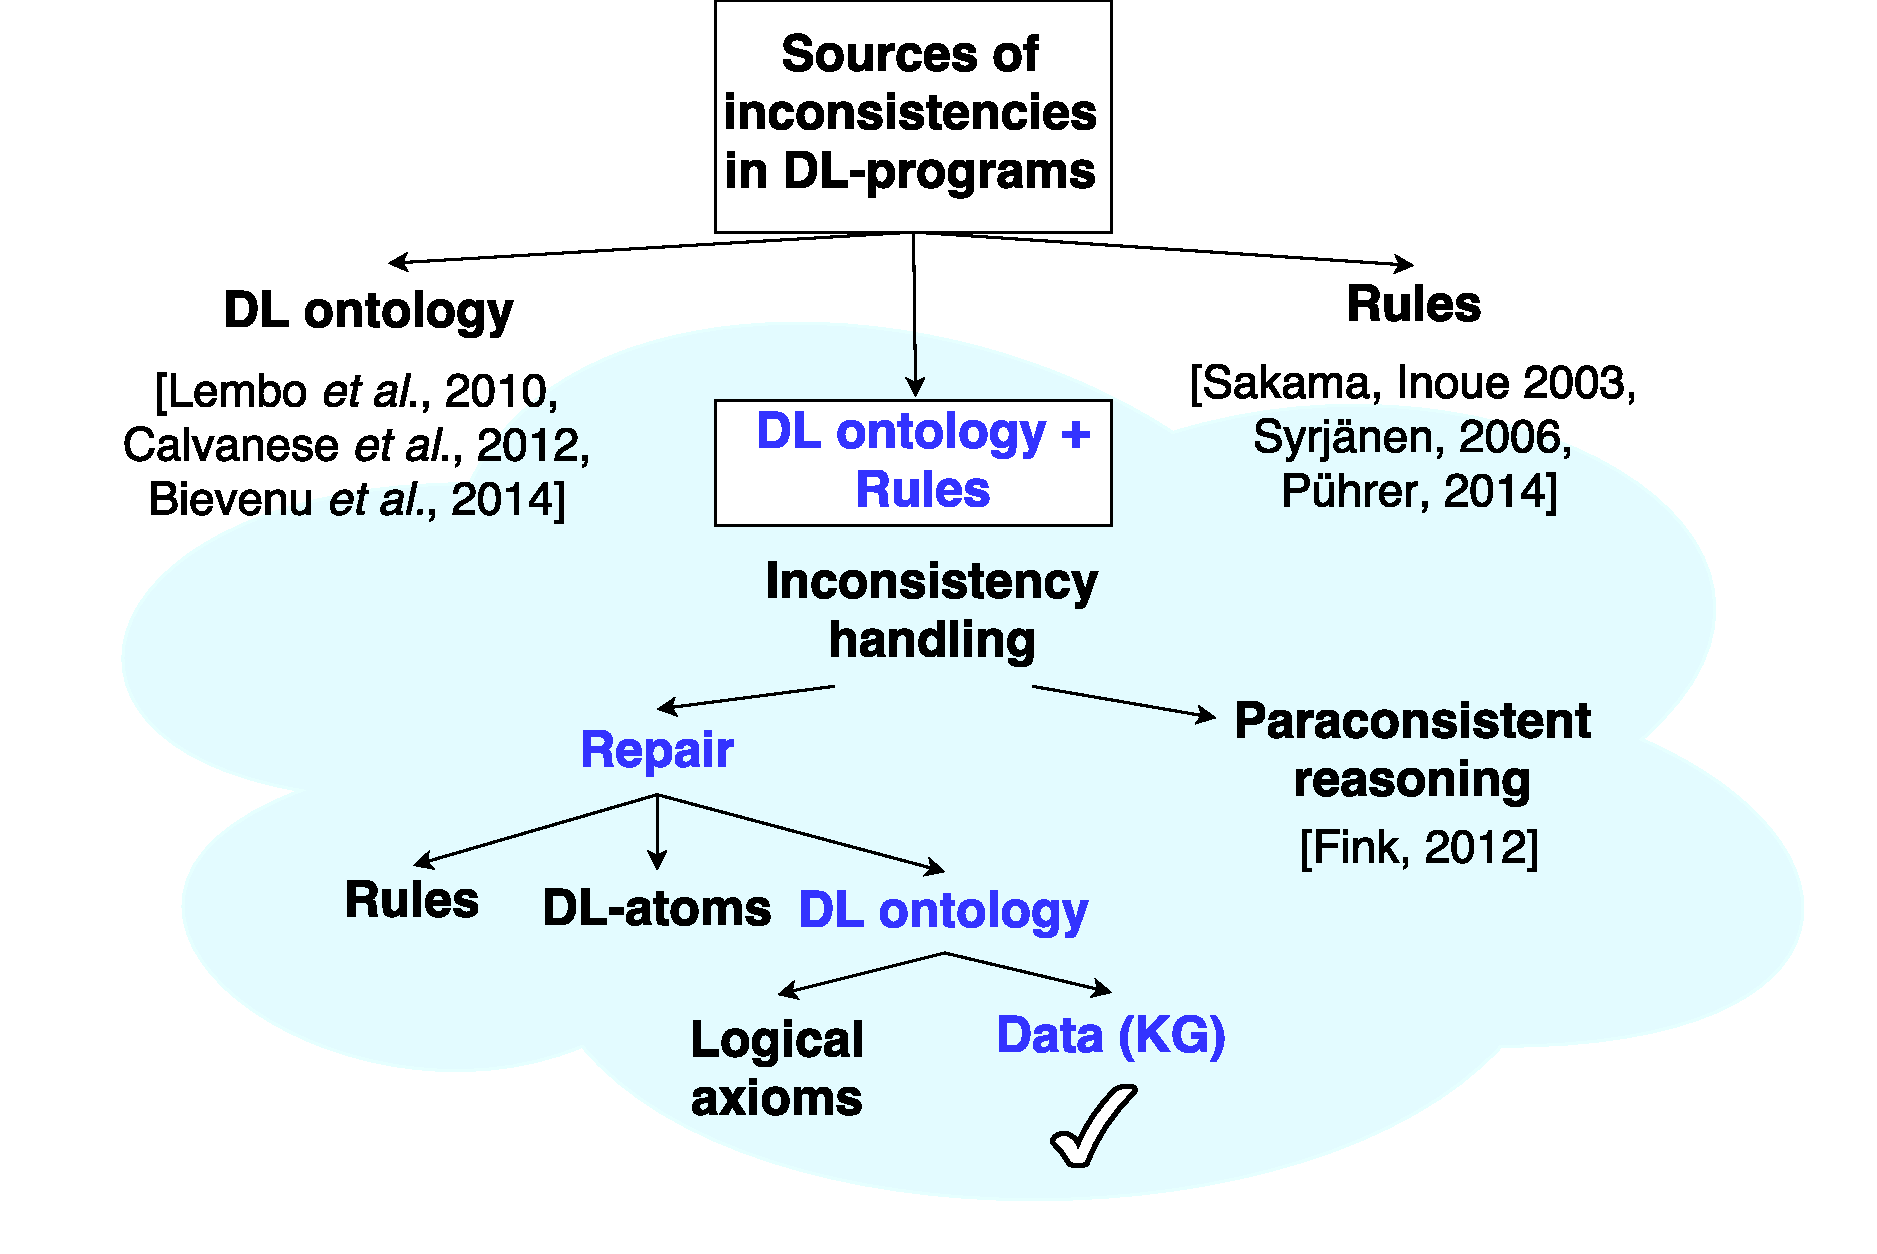
\includegraphics[width=0.9\textwidth]{InconsisDLP}
% \end{center}

% \end{frame}




% \begin{frame}
% \frametitle{Complexity of Repair Answer Sets}
% \bigskip

% \begin{tabular}{|l|}
% \hline
% \small{\textbf{INSTANCE}: A ground DL-program $\Pi=\tuple{O,P}$.}\\
% \small{\textbf{QUESTION}: Does there exist a repair answer set for $\Pi$?} \\
% \hline
% \end{tabular}
% \bigskip

% \begin{theorem}
%  Deciding repair and standard answer set existence have the same complexity if instance query-answering in $O$ is polynomial ($\dllite_{\cA}, \el$).
%  \end{theorem}

% \begin{table}[ht]

% \centering 

% \begin{tabular}{| c | c | c |} 
% \hline
% \centering{\bl{$\Pi$}} & \bl{FLP semantics}& \bl{weak semantics}\\ [0.5ex] % inserts table
% %heading
% \hline 
% \bl{normal} &  \small{$\Sigma^P_2$-complete} &  \small{$\NP$-complete}\\ [1.5ex]% inserting body of the table
% \hline
% \bl{disjunctive} &  \small{$\Sigma^P_2$-complete}&  \small{$\Sigma^P_2$-complete}\\
% [1.5ex] 
% \hline
% \end{tabular}
% \label{table:nonlin} 
% \end{table}
% \bigskip
% \bigskip
% \bigskip


% \tiny{T. Eiter, M. Fink, D. Stepanova. Data Repair of Inconsistent DL-programs. \emph{IJCAI2013}}
% \\
% \tiny{T. Eiter, M. Fink, D. Stepanova. Data Repair of Inconsistent Nonmonotonic Description Logic Programs. \emph{JAI2016}}
% \end{frame}



% \begin{frame}\frametitle{Ontology Repair Problem}
% \bigskip

% \begin{tabular}{|l|}
% \hline
% \small{\textbf{INSTANCE}: Ontology $O$, \gr{$D_{\mi{true}}=\{\tuple{\mi{update,query}}\}$}, \alert{$D_{\mi{false}}=\{\tuple{update,query}\}$}}\\
% \small{\textbf{QUESTION}: Does there exist $O$ data part, for which queries under their}\\\phantom{\small{\textbf{QUESTION}:}} \small{updates from $\gr{D_{\mi{true}}}$ are true and from $\alert{D_{\mi{false}}}$ are false?} \\
% \hline
% \end{tabular}
% \bigskip

% \begin{theorem}
%  The Ontology Repair Problem is \NP-complete even if $O=\emptyset$.
%  \end{theorem}
% \bigskip

% \bl{Tractable cases:}
% \begin{itemize}
% \item Deletion repair
% \item Bounded addition
% \item Bounded change
% \item $\dotsc$
% \end{itemize}
% \end{frame}

% \begin{frame}
% \frametitle{Optimized DL-program Repair}

% \small{\begin{itemize}
% \item For each \bl{DL-atom} compute \bl{minimal sets of facts} (\sups), whose presence in ontology \bl{ensures DL-atom's query entailment} (small for some DLs)
% \uncover<2->{\item \bl{Guess values of DL-atoms} under which the program has an answer set}
% \uncover<3->{\item Solve \bl{ontology repair problem} as a variant of a \bl{hitting set problem}}
% \end{itemize}}
% \bigskip
% \bigskip
% \bigskip
% \bigskip
% \bigskip
% \bigskip
% \bigskip
% \bigskip
% \bigskip
% \bigskip
% \bigskip

% \begin{picture}(0.3,0.3)
%    \put(50,-5){\alt<3>{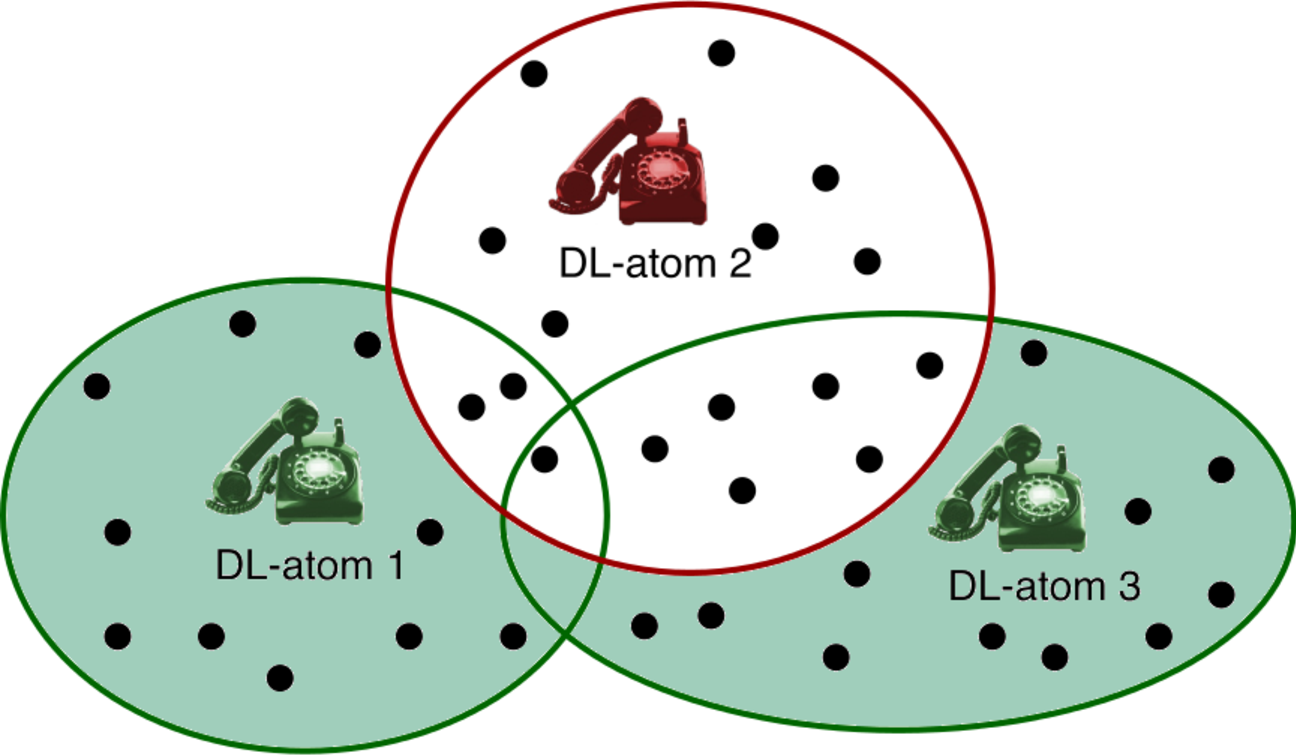
\includegraphics[width=.7\textwidth]{opt3}}{\alt<2>{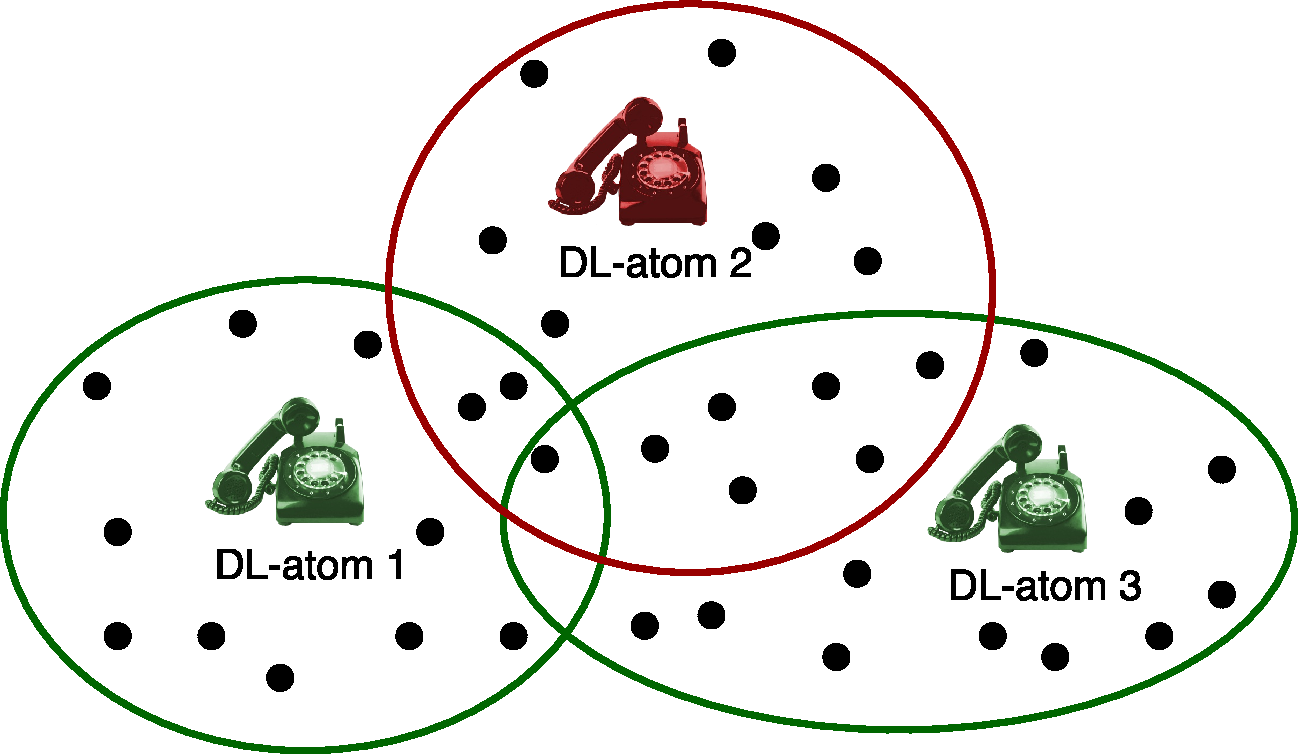
\includegraphics[width=0.7\textwidth]{opt2}}{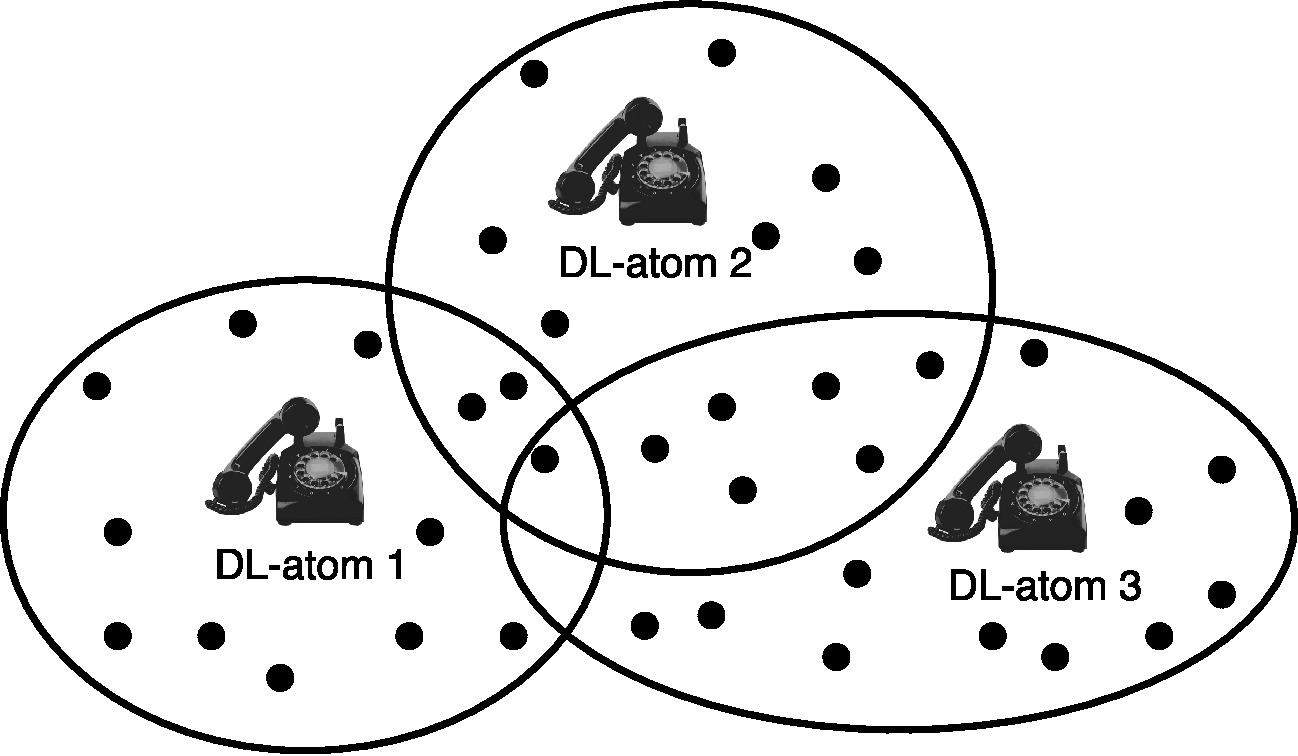
\includegraphics[width=.7\textwidth]{opt1}}}}
% \end{picture}
% \bigskip

% \uncover<3>{
% \tiny{T. Eiter, M. Fink, D. Stepanova. Towards Practical Deletion Repair of Inconsistent
% DL-programs. \emph{ECAI2014}}
% \\
% \tiny{T. Eiter, M. Fink, D. Stepanova. Computing Repairs for Inconsistent DL-programs
% over $\el$ Ontologies. \emph{JELIA2014, JAIR2016}}}

% \end{frame}


% \begin{frame}
% \frametitle{Example Benchmark}
% \begin{picture}(0.3,0.3)
%    \put(220,-30){
\includegraphics[width=0.3\textwidth]{osm}}
% \end{picture}

% \bigskip
% \begin{itemize}
% \item \bl{Ontology:} MyITS\footnote{\tiny{http://www.kr.tuwien.ac.at/research/projects/myits/}}
% \begin{itemize}
% \item \bl{personalized route planning} with semantic
% information
% \smallskip

% \item logical axioms (406), (building features
% located inside private areas are not publicly accessible, covered
% bus stops are those with roofs) 
% \smallskip

% \item KG (4195 facts), Cork city map with leisure areas, bus stops,..
% \end{itemize}
% \bigskip


% \item \bl{Rules:} check that public stations don't lack public access, using \phantom{Rules:} CWA on private areas
% \bigskip

% \item \alert{Inconsistency:} wrong GPS coordinates result in roofed bus stops \phantom{Inconsistency:} being located inside private areas
% \bigskip

% \item \bl{Repair:} found within 12 seconds
% \end{itemize}
% \end{frame}


% \section{Nonmonotonic Rule Mining}


% \begin{frame}
% \frametitle{Overview}
% \begin{itemize}
% \item[$\checkmark$] \bl{Motivation}
% \bigskip

% \item[$\checkmark$] \bl{Ontologies and Rules}
% \bigskip

% \item[$\checkmark$] \bl{Inconsistencies in DL-programs}
% \bigskip

% \item[] \textbf{\bl{Nonmonotonic Rule Mining}}
% \bigskip

% \item[] \bl{Further and Future Work}
% \end{itemize}
% \begin{picture}(0.5,0.5)
% \put(170,45){\includegraphics[width=0.07\textwidth]{moh}}
% \put(163,35){\text{\tiny{M. Gad-Elrab}}}
% \end{picture}

% \begin{picture}(0.5,0.5)
% \put(202,58){\includegraphics[width=0.06\textwidth]{jacoppo}}
% \put(201,48){\text{\tiny{J. Urbani}}}
% \end{picture}

% \begin{picture}(0.5,0.5)
% \put(230,72){\includegraphics[width=0.065\textwidth]{weikum}}
% \put(227,62){\text{\tiny{G. Weikum}}}
% \end{picture}

% %\uncover<2>{
% \begin{picture}(0.5,0.5)
% \put(260,85.5){\includegraphics[width=0.08\textwidth]{tran}}
% \put(260,75.5){\text{\tiny{D. H. Tran}}}
% \end{picture}

% \begin{picture}(0.5,0.5)
% \put(292,98){\includegraphics[width=0.07\textwidth]{lisi}}
% \put(294,88){\text{\tiny{F. A. Lisi}}}
% \end{picture}
% %}
% \end{frame}


% \begin{frame}\frametitle{\alt<4>{Nonmonotonic Rule Mining}{Horn Rule Mining}}
% \smallskip

% \uncover<2->{\alt<4->{\bl{Nonmonotonic rule mining} from KGs: \alert{OWA} is a challenge!}{\bl{Horn rule} mining for KG \bl{completion} \cite{amie} } }
%  \bigskip
%  \bigskip
%  \bigskip
%  \bigskip
%  \bigskip
%  \bigskip
%  \bigskip
%  \bigskip
%  \bigskip
%  \bigskip
%  \bigskip
%  \bigskip
%  \bigskip
%  \bigskip
%  \bigskip
%  \bigskip

% \alt<4->{\begin{picture}(0.5,0.5)\put(43,-33){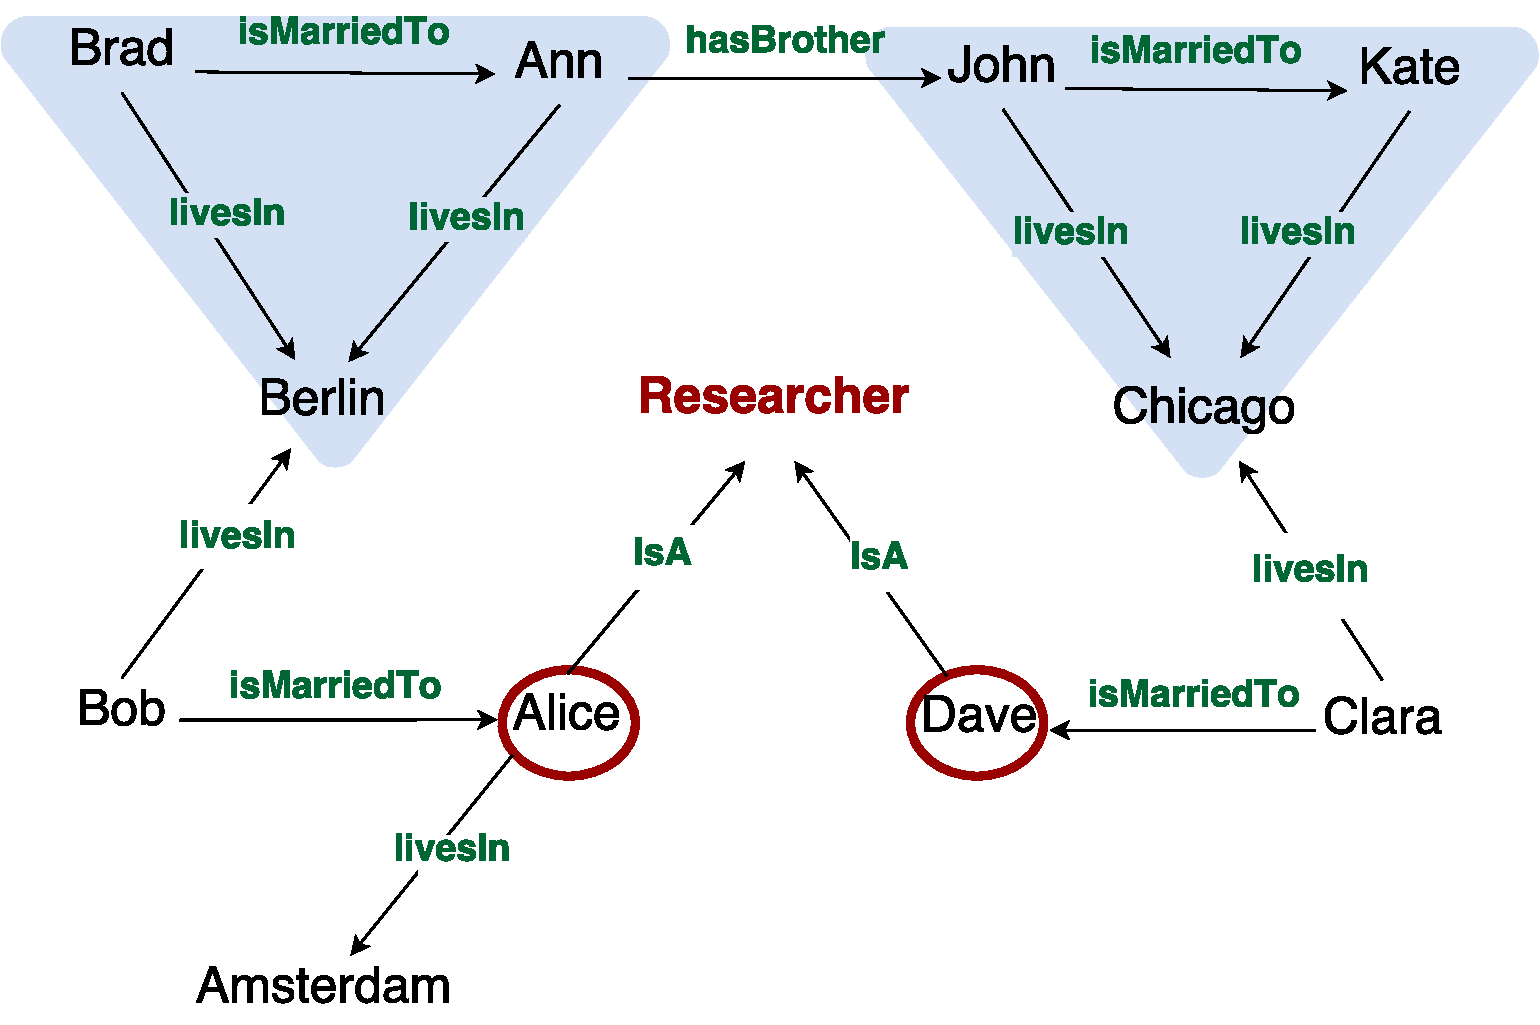
\includegraphics[width=0.75\textwidth]{kg3}}\end{picture}}{
% \alt<3->{
% \begin{picture}(0.5,0.5)\put(43,-33){\includegraphics[width=0.75\textwidth]{kg2}}\end{picture}
% }{\alt<2->{\begin{picture}(0.5,0.5)\put(43,-33){\includegraphics[width=0.75\textwidth]{kg1}}\end{picture}}{\begin{picture}(0.5,0.5)\put(43,-33){\includegraphics[width=0.75\textwidth]{kg0}}\end{picture}}}}
% \begin{center}
% \visible<2->{\rightline{\gr{$\mi{conf(r)}=\dfrac{|\myfilledtriangle{lightblue}|}{|\myfilledtriangle{lightblue}|+|\mytriangle{darkred}{white}|}=$\alt<4>{$1$}{$\dfrac{2}{4}$}}}}
% \bigskip
% \bigskip

% \uncover<2->{\normalsize{\alt<4>{\textcolor{darkgreen}{$r:\;\mi{livesIn(X,Z)}\leftarrow \mi{isMarriedTo(Y,X),livesIn(Y,Z)},$}\,\alert{$\naf\ researcher(X)$}}{\textcolor{darkgreen}{$r:\;\mi{livesIn(X,Z)}\leftarrow \mi{isMarriedTo(Y,X),livesIn(Y,Z)}$}}}}
%  \end{center}

% \end{frame}



% \begin{frame}\frametitle{\alt<2>{Declarative Programming Example}{Declarative Programming Paradigm}}
% \alt<2>{
%  \begin{picture}(0.5,0.5)
%  \put(20,-135){\includegraphics[width=0.9\textwidth]{asp_2}}
%  \end{picture}
% \put(31,65){\text{\small{Graph 3-colorability}}}

% \begin{picture}(0.5,0.5)
% \put(20,115){\includegraphics[width=0.32\textwidth]{graph}}
% \end{picture}
% \begin{picture}(0.5,0.5)
% \put(207,115){\includegraphics[width=0.32\textwidth]{graph_col}}
% \end{picture}
% \put(85,70){$
% \tiny{
% \begin{array}{@{\,}l@{~\,}}
% \gr{\mi{node(1\dotsc 6)};\;\;\;\;\mi{edge(1,2)};\;\;\;\; \dotsc}\\[0.35ex]
% \gr{\mi{col(V,red)}\leftarrow \naf\;\mi{col(V,blue)}, \naf\;\mi{col(V,green)},\mi{node(V)};}\\[0.35ex]
% \gr{\mi{col(V,green)}\leftarrow \naf\;\mi{col(V,blue)},\naf\;\mi{col(V,red)},\mi{node(V)};}\\[0.35ex]
% \gr{\mi{col(V,blue)}\leftarrow \naf\;\mi{col(V,green)},\naf\;\mi{col(V,red)},\mi{node(V)};}\\[0.35ex]
% \gr{\bot\leftarrow \mi{col(V,C)},\mi{col(V,C')},C \neq C';}\\[0.35ex]
% \gr{\bot \leftarrow \mi{col(V,C)},\mi{col(V',C)}, \mi{edge(V,V')}}\\[0.35ex]
% \end{array}}
% $}
%  \put(215,0){\tiny{$\begin{array}{@{\,}l@{~\,}}
% \gr{\mi{node(1\dotsc 6)}};\;\;\;\;\gr{\mi{edge(1,2)};\dotsc}\\ \gr{\mi{col(1, red),col(2,blue)},}\\ \gr{\mi{col(3,red),col(4,green)},}\\ \gr{\mi{col(6,green),col(5,blue)}}\end{array}$}}
% }{
% \begin{picture}(0.5,0.5)
% \put(20,-120){\includegraphics[width=0.86\textwidth]{asp_1}}
% \end{picture}
% }
% \end{frame}

% \begin{frame}\frametitle{Nonmonotonic Rule Mining}
% \alt<2>{\begin{picture}(0.5,0.5)
% \put(20,-190){\includegraphics[width=0.86\textwidth]{asp_4}}
% \end{picture}

% \begin{picture}(0.5,0.5)
% \put(209,-35){\includegraphics[width=0.258\textwidth]{kg0}}
% \end{picture}
% \put(26,-138){\gr{\tiny{$\begin{array}{@{\,}l@{~\,}}
% \mi{livesIn(Y,Z)}\leftarrow \mi{isMarried(X,Y)}, \\
% \phantom{\mi{livesIn(Y,Z)}\leftarrow} \mi{livesIn(X,Y)}, \\ \phantom{\mi{livesIn(Y,Z)}\leftarrow}\naf\ \mi{researcher(Y)}\end{array}
% $}}}
%  \put(209,-138){\gr{\tiny{$\begin{array}{@{\,}l@{~\,}}
% \mi{\gr{isMarriedTo}(brad,ann)};\\ \mi{\gr{isMarriedTo}(john,kate)};\\ \mi{\gr{isMarriedTo}(bob,alice)};\\ \mi{\gr{isMarriedTo}(clara, dave)}; \\ \mi{\gr{livesIn}(brad,berlin};\\ \dotsc\\ \mi{researcher(alice)};\\ \mi{researcher(dave)}\end{array}$}}}
% }{\begin{picture}(0.5,0.5)
% \put(20,-120){\includegraphics[width=0.86\textwidth]{asp_3}}
% \end{picture}}
% \end{frame}

% \begin{frame}\frametitle{Nonmonotonic Rule Mining from KGs}
% \bl{\textbf{Goal:}} learn nonmonotonic rules from KG\\
% \bl{\textbf{Approach:}} revise association rules learned using data mining methods
% \medskip

% \includegraphics[width=1.02\textwidth]{nmlearn}

% \end{frame}


% \begin{frame}\frametitle{Horn Theory Revision}
% \bigskip

%  \begin{beamerboxesrounded}[upper=uppercolblue,lower=lowercolblue,shadow=true]{\textbf{\bl{Quality-based Horn Theory Revision}}}

%  \smallskip

%  \textbf{Given:} 
%  \begin{itemize}
%  \item Available KG 
% \uncover<2->{ \item Horn rule set}
%  \end{itemize}

% \bigskip
% \bigskip
% \bigskip
% \bigskip
% \bigskip

%  \uncover<3->{\noindent \textbf{Find:} }
%  \begin{itemize}
% \uncover<3->{ \item Nonmonotonic revision of Horn rule set}\uncover<4->{\\ with better 
%  predictive quality}
%  \end{itemize}
%  \end{beamerboxesrounded}
% \begin{picture}(0.5,0.5)\put(143,45){\alt<4>{\includegraphics[width=0.58\textwidth]{big_pic_4}}{\alt<3>{\includegraphics[width=0.58\textwidth]{big_pic_3}}{\alt<2>{\includegraphics[width=0.58\textwidth]{big_pic_2}}{\includegraphics[width=0.58\textwidth]{big_pic_1}}}}}\end{picture}
% \end{frame}

% \begin{frame}\frametitle{Avoid Data Overfitting}
% \begin{beamerboxesrounded}[upper=uppercolgreen,lower=lowercolgreen,shadow=true]{How to distinguish exceptions from noise?}\bigskip

% \small{$
%             \renewcommand{\arraystretch}{1.1}
%              \begin{array}{@{\,}l@{~~}l@{}}
%                \mi{\gr{r1:\,livesIn(X,Z) \leftarrow isMarriedTo(Y,X),livesIn(Y,Z),}\, \alert{\naf\ researcher(X)}}\\
%               \visible<2->{\phantom{r1:\,}\mi{\,not\_livesIn(X,Z) \leftarrow isMarriedTo(Y,X),livesIn(Y,Z),researcher(X)}\\[2.75ex]}
%               \visible<3->{\mi{\gr{r2:\,livesIn(X,Z)\leftarrow bornIn(X,Z),\,}\alert{\naf\ moved(X)}}}\\
%               \visible<3->{\phantom{r1:\,}\mi{\,not\_livesIn(X,Z)}\leftarrow bornIn(X,Z),moved(X)}
%              \end{array}$\bigskip

% \uncover<4>{$\{\gr{\mi{livesIn(c,d)}},\mi{not\_livesIn(c,d)}\}$ are conflicting predictions\bigskip

% \textbf{Intuition:} Rules with good exceptions should make few conflicting predictions
% }}
% \end{beamerboxesrounded}
% \end{frame}

% \begin{frame}\frametitle{Horn Theory Revision}

% \bigskip

%  \begin{beamerboxesrounded}[upper=uppercolblue,lower=lowercolblue,shadow=true]{\textbf{\bl{Quality-based Horn Theory Revision}}}

%  \smallskip

%  \textbf{Given:} 
%  \begin{itemize}
%  \item Available KG 
%  \item Horn rule set
%  \end{itemize}

% \bigskip
% \bigskip
% \bigskip
% \bigskip
% \bigskip

%  \noindent \textbf{Find:} 
%  \begin{itemize}
%  \item Nonmonotonic revision of Horn rules, such that \\
% \begin{itemize}
% \item number of \bl{conflicting predictions} is \textbf{minimal} \smallskip

% \item average \bl{conviction}
% is \textbf{maximal}
% \end{itemize}
%  \end{itemize}
%  \end{beamerboxesrounded}
% \begin{picture}(0.5,0.5)\put(143,68){\includegraphics[width=0.58\textwidth]{big_pic_4}}\end{picture}
% \end{frame}


% \begin{frame}\frametitle{Exception Candidates}
% \begin{picture}(0.5,0.5)\put(40,-183,5){\includegraphics[width=0.75\textwidth]{kg_advanced3}}
% \end{picture}
% \bigskip
% \bigskip
% \bigskip
% \bigskip
% \bigskip
% \bigskip
% \bigskip
% \bigskip
% \bigskip
% \bigskip
% \bigskip
% \bigskip
% \bigskip
% \bigskip
% \bigskip
% \bigskip
% \bigskip


% \leftline{\gr{$r{:}\,\mi{livesIn(X,Z)}\,{\leftarrow}\, \mi{isMarriedTo(Y,X)\,{,}\,livesIn(Y,Z)}$}}
% \FrameText{\alert{$\left\{\begin{array}{@{}l@{}}
%  \mbox{}\small{\mi{{\naf}\,researcher(X)}}\\
% \mbox{}\small{\mi{{\naf}\,artist(Y)}}\end{array}\right\}$}}
% \end{frame}



% \begin{frame}\frametitle{Exception Ranking}

% \begin{center}
% $\mi{\gr{rule1}\;\;\; \alert{\{\underline{\mathbf{e_1}},e_2,e_3, \dotsc\}}}$\\
%  $\mi{\gr{rule2}\;\;\; \alert{\{e_1,\underline{\mathbf{e_2}},e_3, \dotsc\}}}$\\
%  $\mi{\gr{rule3}\;\;\; \alert{\{\underline{\mathbf{e_1}},e_2,e_3, \dotsc\}}}$\\
% \end{center}

% \begin{beamerboxesrounded}[upper=uppercolred,lower=lowercolred,shadow=true]{}
% \small{Finding globally best revision is expensive, exponentially many candidates!}
% \end{beamerboxesrounded}
% \begin{itemize}


% \item \bl{Naive ranking:} for every rule inject exception that results in the highest conviction
% \medskip

% \item \bl{Partial materialization (PM):} apply all rules apart from a given one, inject exception that results in the highest average conviction of the rule and its rewriting


% \medskip

% \item \bl{Ordered PM (OPM):} same as PM plus ordered rules application
% \medskip

% \item \bl{Weighted OPM:} same as OPM plus weights on predictions
% \end{itemize}
% \bigskip

% \tiny{M. Gad-Elrab, D. Stepanova, J. Urbani, G. Weikum. Exception-enriched Rule Learning from Knowledge Graphs. \emph{ISWC2016}}\\
% \tiny{D. Tran{,}\,D. Stepanova{,}\,M. Gad-Elrab{,}\,F. Lisi{,}\,G. Weikum. Towards Nonmonotonic Relational Learning from KGs{.}\,\emph{ILP2016}}
% \end{frame}

% \begin{frame}\frametitle{Experimental Setup}
% \vspace{-.4cm}
% \begin{itemize}
% \item \bl{Approximated ideal KG}: original KG 
% \smallskip

% \item \bl{Available KG}: for every relation randomly remove 20\% of facts from approximated ideal KG
% \smallskip

% \item \bl{Horn rules}: $\mi{h(X,Y)\leftarrow p(X,Z),q(Z,Y)}$ 
% \smallskip

% \item \bl{Exceptions}: $\mi{e_1(X),e_2(Y),e_3(X,Y)}$
% \smallskip

% \item \bl{Predictions} are computed using \bl{answer set solver} DLV % \footnote{\tiny{\url{http://dlvsystem.com}}}
% \end{itemize}
% \bigskip
% \bigskip
% \bigskip
% \bigskip
% \bigskip
% \bigskip
% \bigskip
% \bigskip
% \bigskip
% \bigskip
% \bigskip

% \bigskip
% \bigskip

% \visible<1>{\begin{picture}(0.5,0.5)\put(55,63){\includegraphics[width=0.75\textwidth]{big_pic_exp}}
% \end{picture}}

% \visible<2>{\vspace{-5,5cm}\begin{beamerboxesrounded}[upper=uppercolgreen,lower=lowercolgreen,shadow=true]{\textbf{Examples of revised rules:}}

%  \begin{tabular}{l}
% \footnotesize{

% Plots of films in a sequel are written by the same writer, unless a film is American}\\
%         \footnotesize{$\gr{r_1:  \mi{writtenBy(X, Z)}  \leftarrow
%         \mi{hasPredecessor(X, Y)},\mi{writtenBy(Y, Z)},}$ \alert{$ not$  $\mi{american\_film(X)} $}}\\   
% \\     
% \footnotesize{
% Spouses of film directors appear on the cast, unless they are silent film actors
% }\\
%       \footnotesize{ 
% $\gr{r_2:  \mi{actedIn(X, Z)}  \leftarrow
%         \mi{isMarriedTo(X, Y)},\mi{directed(Y, Z)},}$ \alert{$ not$  $\mi{silent\_film\_actor(X)} $}} \\
    
%  \end{tabular} 
% \end{beamerboxesrounded}      }



% \end{frame}

% \section{Ongoing and Future Work}
% \begin{frame}\frametitle{Overview}
% \begin{itemize}
% \item[$\checkmark$] \bl{Motivation}
% \bigskip

% \item[$\checkmark$] \bl{Ontologies and Rules}
% \bigskip

% \item[$\checkmark$] \bl{Inconsistencies in DL-programs}
% \bigskip

% \item[$\checkmark$] \bl{Nonmonotonic Rule Mining}
% \bigskip

% \item[] \textbf{\bl{Ongoing and Future Work}}
% \end{itemize}
% \end{frame}



% \begin{frame}\frametitle{Completeness-aware Rule Mining}
% \begin{itemize}
% \item Exploit \bl{cardinality meta-data} \cite{card} in \bl{rule mining}\\
% \emph{\gr{John has \textbf{5} children, Mary is a citizen of \textbf{2} countries}}
% \end{itemize}
% \bigskip\bigskip
% \bigskip
% \bigskip
% \bigskip
% \bigskip
% \bigskip
% \bigskip
% \bigskip
% \bigskip
% \bigskip

% \begin{picture}(0.5,0.5)\put(40,-26){\includegraphics[width=0.8\textwidth]{worldmap}}
% \end{picture}

% \bigskip
% \bigskip
% \bigskip
% \bigskip

% \tiny{Joint work with T. Pellissier-Tanon, S. Razniewski, P. Mirza, G. Weikum}
% \end{frame}




% \begin{frame}\frametitle{Ongoing and Future Work}
% \begin{itemize}
% \item Make use of \bl{logical background knowledge} in
% \begin{itemize}
% \normalsize{\item \bl{Rule learning} and other \bl{data mining} tasks}\footnote{\tiny{S. Paramonov, D. Stepanova, P. Miettinen. Hybrid Approach to Constraint-based Pattern Mining. Accepted to \emph{RR2017}}}
% \smallskip

% \normalsize{\item \bl{Information extraction} from text corpora}\footnote{\tiny{Joint work with M. Gad-Elrab, J. Urbani, G. Weikum}}
% \smallskip

% \normalsize{\item \bl{Natural language processing} tasks}
% \end{itemize}
% \end{itemize}
% \bigskip
% \bigskip

% \begin{itemize}
% \item Exploit \bl{answer set programs with\\ external computations} \cite{DBLP:conf/frocos/EiterBDFIK09} \\for the above problems
% \end{itemize}

% \begin{picture}(0.5,0.5)
%  \put(230,-20){\includegraphics[width=0.27\textwidth]{hex}}
% \end{picture}
% \end{frame}

% \begin{frame}\frametitle{Conclusion}

% \textbf{\bl{Summary:}}
% \begin{itemize}
% \small{\item \bl{Inconsistencies in combination of rules and ontologies}}
% \begin{itemize}
% \item Repair semantics and its complexity analysis
% \item Optimized algorithms for repair computation \\and their evaluation ($\dllite_{\cA}$ and $\el$ DLs)
% \end{itemize}
% \bigskip

% \small{\item \bl{Nonmonotonic rule mining from KGs}}
% \begin{itemize}
% \item Quality-based Horn theory revision framework under OWA
% \item Approach for computing and ranking exceptions based on\\ cross-talk among rules and its evaluation on real-world KGs
% \end{itemize}
% \end{itemize}
% \bigskip
% \bigskip

% \textbf{\bl{Future Directions:}}
% \small{\begin{itemize}
% \item Interlinking mining and reasoning in the KG context
% \item Exploiting logical background knowledge in information \\extraction and natural language processing tasks
% \end{itemize}}

% \end{frame}


% \appendix
% \begin{frame}[plain,allowframebreaks,allowdisplaybreaks]
%   \frametitle{References}
%   \bibliographystyle{named}
%  \tiny{\bibliography{references}}
% \end{frame}
% \section{Additional Material}


% \begin{frame}
% \frametitle{DL-program Repair Algorithm}
% \vspace{-.15cm}
% \begin{center}
% \alt<9->{\includegraphics[width=0.87\textwidth]{DLP_algfinalfail}}{\alt<8>{\includegraphics[width=0.87\textwidth]{DLP_algfinalok}}{\alt<7>{\includegraphics[width=0.87\textwidth]{DLP_alg5b}}{\alt<6>{\includegraphics[width=0.87\textwidth]{DLP_alg5a}}{\alt<5>{\includegraphics[width=0.87\textwidth]{DLP_alg4}}{\alt<4>{\includegraphics[width=0.87\textwidth]{DLP_alg3}}{\alt<3>{\includegraphics[width=0.87\textwidth]{DLP_alg2}}{\alt<2>{\includegraphics[width=0.87\textwidth]{DLP_alg1}}{\includegraphics[width=0.87\textwidth]{DLP_alg0}}}}}}}}}
% \end{center}
% \end{frame}


% \begin{frame}\frametitle{Spurious Rules due to Incompleteness}
% \uncover<2->{\begin{center}\bl{In real world:}\end{center}}
% \alt<3>{\begin{picture}(0.5,0.5)\put(25,-160){\includegraphics[width=0.85\textwidth]{kg_polit3}}
% \end{picture}}{\alt<2>{\begin{picture}(0.5,0.5)\put(25,-160){\includegraphics[width=0.85\textwidth]{kg_polit2}}
% \end{picture}}{\begin{picture}(0.5,0.5)\put(25,-160){\includegraphics[width=0.85\textwidth]{kg_polit1}}
% \end{picture}}}
% \bigskip
% \bigskip
% \bigskip
% \bigskip
% \bigskip
% \bigskip
% \bigskip
% \bigskip
% \bigskip
% \bigskip
% \bigskip
% \bigskip
% \bigskip
% \bigskip
% \bigskip

% \visible<1->{\rightline{\gr{$\mi{conf(r)}=\dfrac{|\myfilledtriangle{lightblue}|}{|\myfilledtriangle{lightblue}|+|\mytriangle{darkred}{white}|}=$\alt<3>{$\dfrac{2}{6}$}{$\dfrac{2}{3}$}}}}
% \bigskip
% \bigskip

% \alt<3>{\centerline{\gr{$\mi{r:\;\overbrace{isPoliticianOf(X,Z)}^{\mi{complete}}}\leftarrow \overbrace{\mi{hasChild(X,Y),isCitizenOf(Y,Z)}}^{\mi{incomplete}}$}}}{\centerline{\gr{$\mi{r:\;isPoliticianOf(X,Z)\leftarrow hasChild(X,Y),isCitizenOf(Y,Z)}$}}}

% \end{frame}


% \begin{frame}\frametitle{Hybrid Constraint-based Pattern Mining}
% \begin{itemize}
% \item Interlink \bl{mining} and \bl{reasoning}
% \item Use declarative \bl{logic programming} \\for frequent pattern (itemset/sequence) filtering
% \item Combine various \bl{domain-specific} constraints 
% \end{itemize}
% \bigskip
% \bigskip
% \bigskip
% \bigskip
% \bigskip
% \bigskip
% \bigskip
% \bigskip
% \bigskip
% \bigskip
% \bigskip



% \begin{picture}(0.5,0.5)\put(40,-10){\includegraphics[width=0.7\textwidth]{constraint_mining}}
% \end{picture}
% \bigskip
% \bigskip

% \tiny{Sergey Paramonov, Daria Stepanova, Pauli Miettinen. Hybrid Approach to Constraint-based Pattern Mining. \emph{RR2017}}
% \end{frame}


% \begin{frame}\frametitle{Semantically-enhanced Fact Spotting}
% \bigskip
% \bigskip

% \textbf{\bl{KG population problem:}} some facts are hard to spot in text due to reporting bias \gr{$\mi{lost(nadal,australianOpen2017)}$} 
% \bigskip
% \bigskip

% \bl{\textbf{Given:}} 
% \begin{itemize}
% \item Fact: \gr{$\mi{lost(nadal,australianOpen2017)}$} 
% \item Rule set: \gr{$\mi{lost(Z,Y)\leftarrow won(X,Y),finalist(Z,Y), X\neq Z}$}
% \item KG:  \gr{$\mi{won(federer,australianOpen2017)}$}
% \item Text: \gr{``... \emph{another \textbf{finalist} of \textbf{Australian Open in 2017} was \textbf{Nadal}}''}
% \end{itemize}
% \bigskip
% \bigskip

% \bl{\textbf{Find:}}
% \begin{itemize}
% \item Fact's truth value: \gr{$\mi{lost(nadal,australianOpen2017)}$} is true!
% \end{itemize} 
% \bigskip
% \bigskip
% \bigskip

% \tiny{Joint work with Mohamed Gad Elrab, Jacopo Urbani and Gerhard Weikum}

% \end{frame}






\end{document}

%%% Local Variables:
%%% TeX-PDF-mode: t
%%% TeX-debug-bad-boxes: t
%%% TeX-master: t
%%% TeX-parse-self: t
%%% TeX-auto-save: t
%%% reftex-plug-into-AUCTeX: t
%%% End:

